\chapter{Topological states of matter}
\label{ch:topo-intro}
In this Chapter, we introduce some notions from the mathematical field of topology in the context of topological states of matter. We focus on non-interacting fermionic systems and treat them in the general framework of band theory in the tight-binding formalism. In the following, we assume the locality of the Hamiltonians (\ie no infinite-range hoppings) and focus on the properties of ground states at zero temperature. As a starting point, we provide a description of fundamental symmetries in quantum mechanics, which are the basis for further considerations. We elaborate on the classification of topological states with respect to ten distinct symmetry classes and substantiate its connection to the edge physics. Finally, we illustrate these concepts in more details using paradigmatic examples of topological phases. In particular, we provide an accessible explanation of topological invariants.

\section{Topological band theory}
Topology is a branch of mathematics that deals with properties of smooth, continuous transformations such as stretching or bending. The geometrical details of objects are then ignored and only global features, characterized by topological invariants, are of interest. For instance, a sphere can be continuously deformed into a cube, hence both objects are said to be topologically equivalent (or homeomorphic). A deformation from a sphere to a torus is, on the other hand, not a smooth procedure as it requires making a hole. 

\begin{figure}
\centering
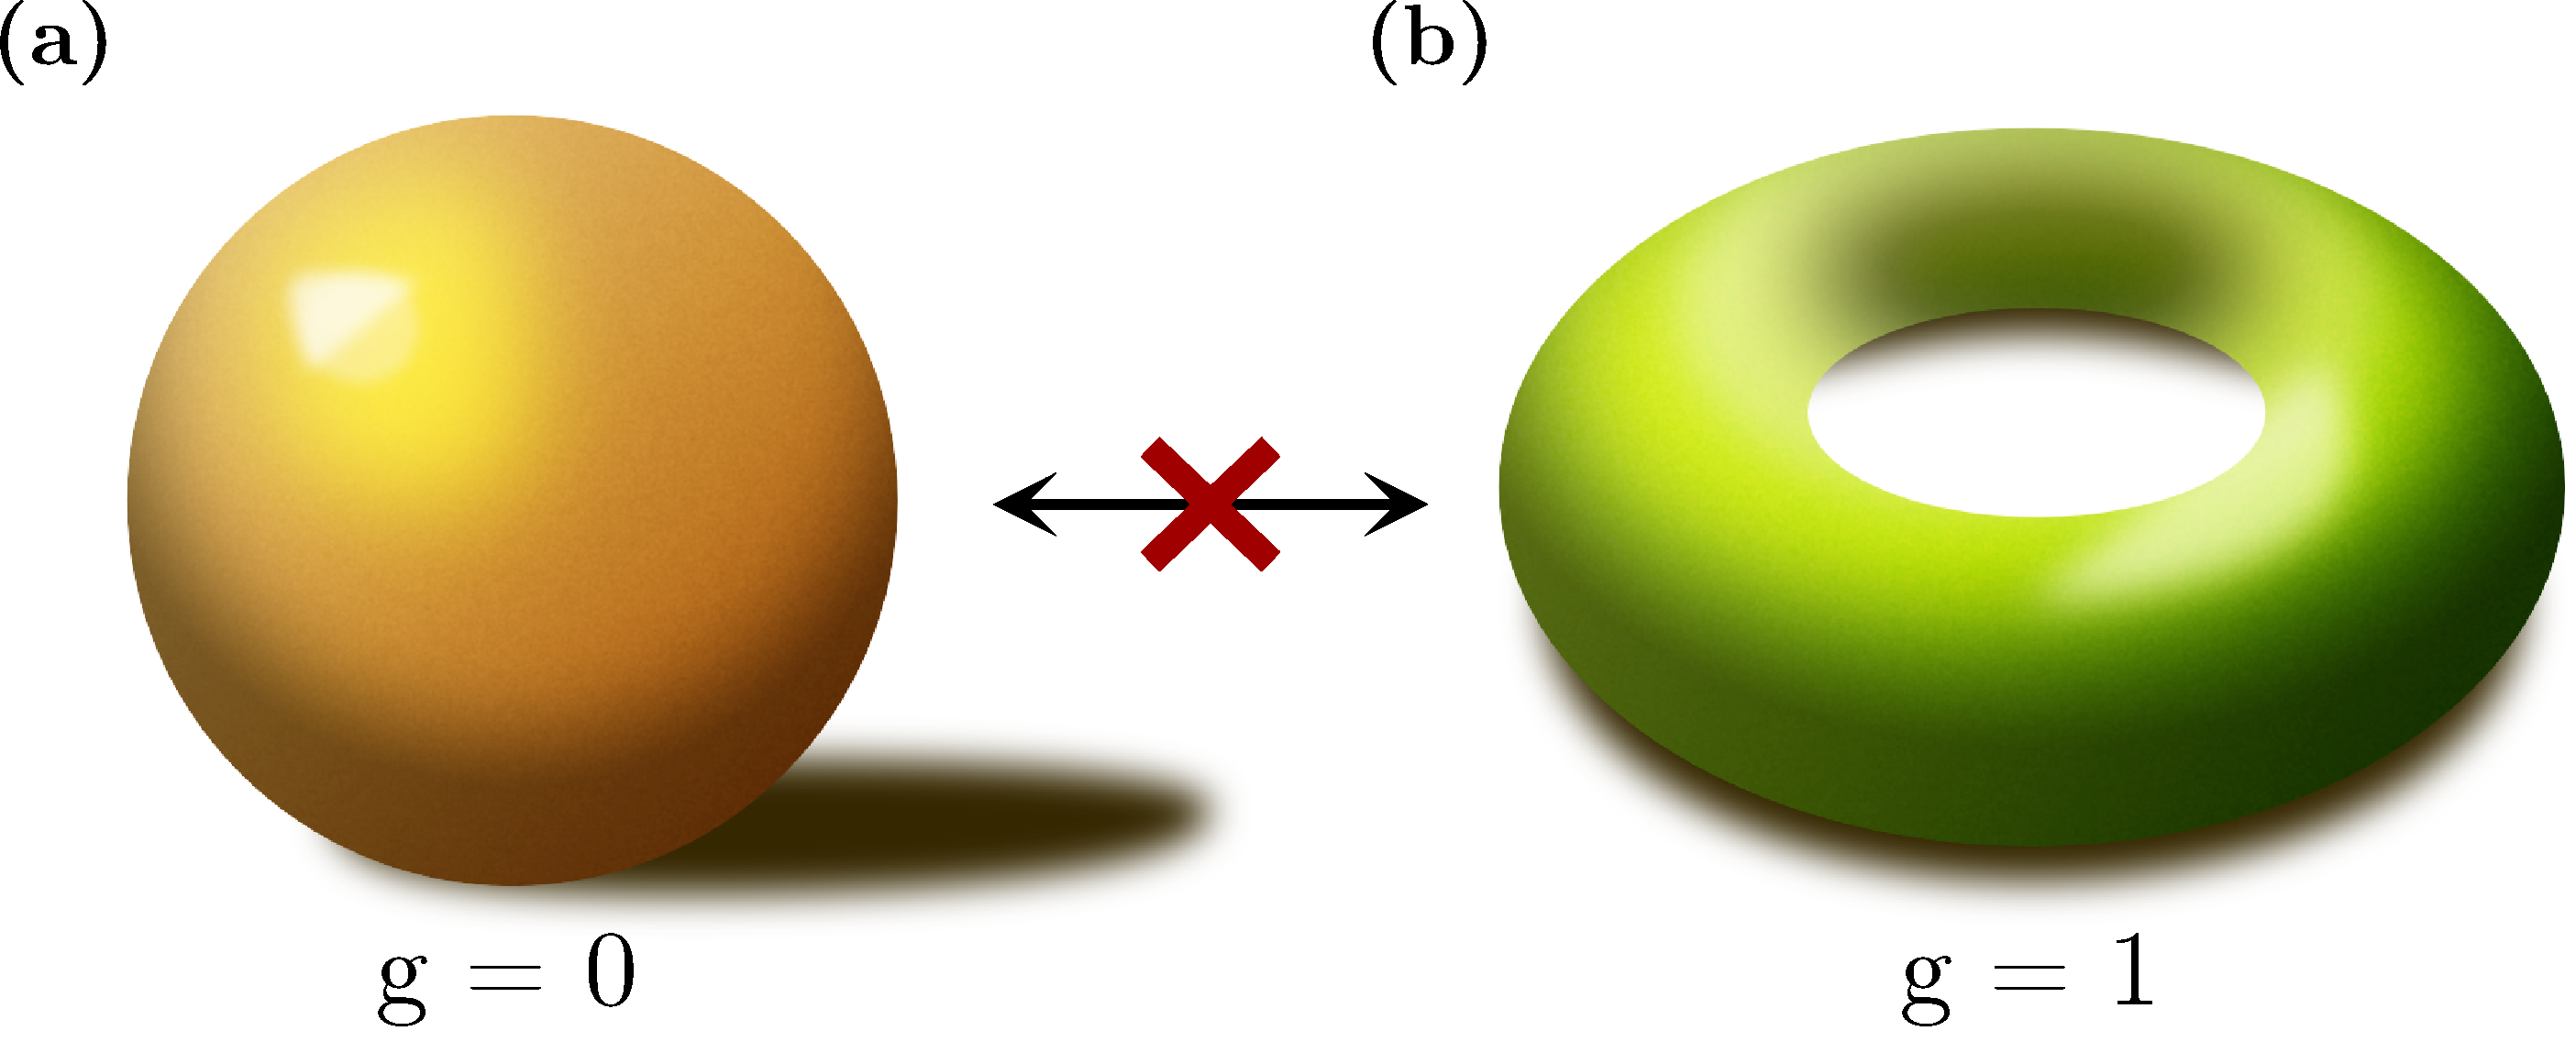
\includegraphics[width = 0.70\textwidth]{intro_sphere-torus.pdf}
\caption[Topological inequivalence]{Topological inequivalence. From a perspective of topology, \textbf{(a)} a sphere and \textbf{(b)} a torus are distinct as one cannot be smoothly deformed into the other. A sphere has a genus $g$ equal to zero, while a torus has one punctured hole and therefore $g = 1$.}
\label{fig:topo_equiv}
\end{figure}

To differentiate between topologically distinct objects, we can assign to each of them the number of holes called the genus $g$. As depicted in Fig.~\ref{fig:topo_equiv}, a sphere is characterized by $g =0$, whereas a torus has $g = 1$. As long as all deformations are smooth, the genus remains unchanged. The criterion for possible smooth deformations is given by the Gauss-Bonnet theorem. In two dimensions, for a given Riemannian manifold $M$ without boundary (\eg a torus), the surface integral of the local Gaussian curvature $K(\mathbf{x})$ is related to the genus $g$ as
\begin{equation}
2 - 2g = \int_{M} K( \mathbf{x}) \, d^2 \mathbf{x}.
\label{eq:gaussbonnet}
\end{equation}
The Gaussian curvature is proportional to the angle mismatch before and after the parallel transport (called holonomy) of a tangent vector enclosing a loop on $M$. 

In the realm of band theory, topological equivalence can be understood by answering the following: Given two band insulators described by Bloch Hamiltonians $\mathcal{H} (\mathbf{k})$ and $\mathcal{H}'(\mathbf{k})$, can we adiabatically deform one to the other without closing the gap? Let us introduce relevant definitions. Quantum lattice free-fermionic models can be described by a Hamiltonian $H$ within a tight-binding approximation, whose most general form reads
\begin{equation}
H = \sum_{ij \alpha \beta} c_{i \alpha}^{\dagger} H_{ij}^{\alpha \beta} c_{j \beta}.
\label{eq:genericTB}
\end{equation}
Here, $i, \, j$ correspond to lattice sites, while $\alpha, \, \beta$ denote internal degrees of freedom such as orbitals or spin. $c_{i \alpha}^{\dagger} ( c_{i \alpha})$ stands for the second-quantized creation (annihilation) operators on sites $i$ and species $\alpha$, which obey the anticommutation relations
\begin{equation}
\lbrace c_{i \alpha}^{\dagger} , c_{j \beta} \rbrace = \delta_{i j}  \delta_{\alpha \beta}, \hspace*{1cm} \lbrace c_{i \alpha}, c_{i \alpha} \rbrace = \lbrace c^{\dagger}_{i \alpha}, c^{\dagger}_{i \alpha} \rbrace  = 0.
\label{eq:commut_rel}
\end{equation}
In the case of a perfectly regular arrangement of sites and with periodic boundary conditions (PBC), the Hamiltonian in Eq.~\eqref{eq:genericTB} can be conveniently represented in reciprocal space. This can be achieved by performing the Fourier transform of the operators
\begin{equation}
 c_{i \alpha} = \frac{1}{\sqrt{V}} \sum_{\mathbf{k} \in \mathrm{BZ}} c_{\mathbf{k} \alpha} \,  e^{\mathrm{i} \mathbf{k} \cdot \mathbf{r}}, \hspace*{1cm} c_{\mathbf{k} \alpha} = \frac{1}{\sqrt{V}} \sum_{\mathbf{r}} c_{i \alpha} \, e^{-\mathrm{i} \mathbf{k} \cdot \mathbf{r}}, 
\label{eq:fourier}
\end{equation}
where $\mathbf{r}$ describes the position of the $i$-th site and $V$ is a volume of the $d$-dimensional system, $V = L^d$. Thus, the momentum-space Hamiltonian is
\begin{equation}
\mathcal{H}= \sum_{\mathbf{k} \alpha \beta} c^{\dagger}_{\mathbf{k} \alpha} \mathcal{H}^{\alpha \beta} (\mathbf{k}) c_{\mathbf{k} \beta}
\label{eq:genericTB_kspace}
\end{equation}
with a size given by the total number of degrees of freedom in the unit cell $N$. $\mathbf{k}$ is the momentum defined in the Brillouin zone (BZ). In the thermodynamic limit (with $L \rightarrow \infty$), the BZ is topologically equivalent to a torus $\mathbf{k} \in T^d$. $\mathcal{H} (\mathbf{k})$ can therefore be seen as a map from $T^d$ to the set of $N \times N$ Hermitian matrices, which we denote by $\mathrm{Hn} (N)$
\begin{equation}
\begin{aligned}
\mathcal{H}: T^d & \rightarrow \mathrm{Hn} (N), \\
\mathbf{k} & \mapsto \mathcal{H} (\mathbf{k}).
\end{aligned}
\end{equation}
The band structure refers to the eigenspectrum $\lbrace \epsilon_a \rbrace$ of $\mathcal{H} (\mathbf{k})$ at every $\mathbf{k}$, \ie, the energy bands. In fermionic systems, a ground state generally forms a Fermi sea due to the Pauli exclusion principle. If there is a spectral gap between $n$ lowest eigenvalues (the occupied energy bands) and the remaining $m$ (empty bands) with $N = n + m$  for $\forall \mathbf{k} \in \mathrm{BZ}$, then the system is said to be \emph{gapped} at filling $n/N$. In contrast, the system is \emph{gapless} if this spectral gap vanishes, namely there exists a shared eigenvalue between the bands $n$ and $n + 1$ in the Brillouin zone.

\subsection{Flat band Hamiltonian}
\label{sec:flatband}
Topological classification is based on the global properties of band structures. As long as the Bloch Hamiltonian $\mathcal{H} (\mathbf{k})$ has a finite gap separating occupied and unoccupied states, it can be continuously deformed to the spectrally flattened Hamiltonian $\mathcal{Q} (\mathbf{k})$. This deformation removes the system-dependent information about the energies, but leaves topological properties intact. We focus on an illustrative example of an insulating system without any symmetries.

The Hamiltonian $\mathcal{H} (\mathbf{k})$ can be diagonalized at every $\mathbf{k} \in \mathrm{BZ}$ using a unitary transformation $U(\mathbf{k})$, 
$U^{\dagger}( \mathbf{k}) \mathcal{H} (\mathbf{k}) U (\mathbf{k}) = \mathrm{diag} \left(\epsilon_N, \, \epsilon_{N-1}, \,  \ldots, \, \epsilon_1 \right)$, where the eigenenergies $\epsilon_a$ are sorted in a descending order. We assume that $n$ out of $N$ bands are occupied, which is equivalent to setting the chemical potential between the bands $n$ and $n + 1$. The \emph{flat band Hamiltonian} $\mathcal{Q} (\mathbf{k})$ reads 
\begin{equation}
\mathcal{Q} (\mathbf{k}) =
U (\mathbf{k}) 
\begin{pmatrix}
\mathbb{1}_m & 0 \\
0 & - \mathbb{1}_n
\end{pmatrix} U^{\dagger} (\mathbf{k})  ; \hspace*{0.5cm} \mathcal{Q}^2(\mathbf{k}) = 1
\label{eq:flatband}
\end{equation}
and its energies are either $-1$ for all occupied bands or $+1$ for states above the gap. In general, $\mathcal{Q} (\mathbf{k})$ is a $\mathrm{U}(m + n)$ matrix with an extra $\mathrm{U} (n) \times \mathrm{U} (m)$ gauge symmetry due to independent basis rotations in the occupied and unoccupied eigenspaces, respectively. If these conditions are taken into account, the flattened and original Hamiltonians belong to the coset space known as the complex Grassmannian $G_{m,n} ( \mathbb{C})$. The set of topologically distinct Hamiltonians $\mathcal{H}$ is given by the homotopy classes of the mappings
\begin{equation}
\begin{aligned}
\mathcal{Q}: \mathrm{BZ} \rightarrow G_{n+ m, \, m} & ( \mathbb{C})  = \frac{\mathrm{U} (n +m) }{\mathrm{U} (n) \times \mathrm{U}(m) }, \\ 
\mathbf{k} \mapsto & \mathcal{Q} (\mathbf{k}).
\end{aligned}
\end{equation}
In the continuum case, the BZ corresponds to the $d$-sphere $S^d$, while for lattice models -- to the $d$-dimensional torus $T^d$. The fact that two maps $k \mapsto & \mathcal{Q} (\mathbf{k})$ and $k \mapsto & \mathcal{Q}' (\mathbf{k})$ can be adiabatically deformed into each other (\eg by changing the model parameters) implies that the corresponding Hamiltonians $\mathcal{H} (\mathbf{k})$ and $\mathcal{H}' (\mathbf{k})$ are \emph{topologically equivalent} and can be smoothly transformed into each other \emph{without} closing the gap. In other words, any continuous transformation that preserves the gap does not change the topology of $\mathcal{H}$. The number of topologically distinct Hamiltonians $\mathcal{H}$ is given by the homotopy group\footnote{Although the homotopy group uses a sphere as the base space for the mappings, the topological classification discussed in this Chapter is most often not affected if the BZ is a torus. In the special cases where this distinction is relevant, the corresponding system is actually a \emph{weak} topological insulator requiring additional spatial symmetries to protect edge modes.} $\pi_d (G_{m, \, n} ( \mathbb{C}))$~\cite{Nakahara}
\begin{equation}
\begin{aligned}
\pi_d (G_{m, \, n} ( \mathbb{C})) &= \mathbb{Z}, \hspace*{0.1cm} d \textnormal{ even}; \\
\pi_d (G_{m, \, n} ( \mathbb{C})) & = \lbrace 1 \rbrace, \hspace*{0.1cm} d \textnormal{ odd}.
\end{aligned}
\end{equation}
This result states that in two (and any other even) dimensions, there is an infinite number of topologically distinct states labeled by an integer \emph{topological invariant}. It is exactly the case of the integer quantum Hall effect, which we discuss in Section~\ref{sec:iqhe}. Conversely, all non-interacting fermionic Hamiltonians in odd dimensions without imposed symmetries are topologically equivalent. In general, the system is said to be \emph{trivial} if it is adiabatically connected to an ordinary insulator of isolated atoms. A deformation leading from a Hamiltonian to another one in a distinct topological class has to pass through a gap closing. The system is then said to undergo a \emph{topological phase transition}.

\subsection{Internal symmetries}
The set of possible deformations that keep the systems adiabatically connected can be further constrained by the presence of symmetries. This gives rise to the notion of \emph{symmetry-protected topological states}, which cannot be deformed into a trivial state unless the gap closes or a relevant symmetry is broken. According to Wigner's theorem~\cite{wigner2013group}, any symmetry in quantum mechanics can be represented by an operator that preserves the inner product and therefore the transition probabilities. Hence, an operator $S$ representing a symmetry has to be either linear and unitary
\begin{equation}
\braket{ S \psi, S ( \lambda_1 \phi_1 + \lambda_2 \phi_2 )} = \lambda_1 \braket{\psi, \phi_1} + \lambda_2 \braket{\psi, \phi_2}
\label{eq:s-linear}
\end{equation}
or antilinear and antiunitary
\begin{equation}
\braket{ S\psi, S( \lambda_1 \phi_1 + \lambda_2 \phi_2 )} = \lambda_1^*  \braket{\phi_1, \psi} + \lambda_2^* \braket{\phi_2, \psi}.
\label{eq:s-antilinear}
\end{equation}
An operator $S$ is a symmetry of the system if it commutes with the Hamiltonian $H$
\begin{equation}
[H, S] = 0.
\end{equation}
Moreover, any antiunitary transformation $S$ can be written as the product of a unitary transformation $U$ and the complex conjugation operator $\mathcal{K}$
\begin{equation}
S = U \mathcal{K}
\label{eq:anti}.
\end{equation}
A unitary symmetry allows to represent the Hamiltonian in a block-diagonal form and reduce the problem to the independent study of each separate block. Antiunitary symmetries, however, are more interesting as they impose certain spectral constraints on the irreducible blocks of the Hamiltonian. Here, we focus on \emph{internal} symmetries acting locally in real space.

A fundamental antiunitary operator is the time-reversal symmetry $\mathcal{T}$ (TRS), which takes the time $t \rightarrow -t$ and reverses the time-evolution $\mathcal{T} e^{-\mathrm{i} t H} \mathcal{T}^{-1} = e^{\mathrm{i} t H}$
\begin{equation}
 \hspace*{0.5cm}  \mathcal{T}  H \mathcal{T}^{-1} = + H.
\label{eq:TRS}
\end{equation}
%\footnote{The $\mathrm{U}(1)$ gauge freedom means that $\ket{\psi}$ and $e^{\mathrm{i} \phi} \ket{\psi}$, $\phi \in \mathbb{C}$ describe the same quantum state.} 
The $\mathcal{T}$ operator belongs to a class of involutional operators, which leave an arbitrary state $\ket{\psi}$ unchanged up to a phase factor when applied twice, $\mathcal{T}^2 = e^{\mathrm{i} \phi} \, \mathbb{1} $. By defining $\mathcal{T} = T \mathcal{K}$ with $T$ being unitary, $T^{-1} = T^{\dagger} = (T^{\mathrm{T}})^*$, one can show that $\mathcal{T}^2 = T \mathcal{K} T \mathcal{K} = T T^*$ and $\mathcal{T}^2 = \eta \, \mathbb{1} = T (T^{\mathrm{T}})^{-1}$ as $T^* = (T^{\mathrm{T}})^{-1}$. Hence, $T= \eta T^{\mathrm{T}} = \eta^2 T$, which implies that $\eta = \pm 1$ and $\mathcal{T}^2 $ may give either $+1$ or $-1$. To show that more explicitly, let us take a spin$-1/2$ system as an example. We can write the TRS operator in the $\sigma_z$ basis as
\begin{equation}
\mathcal{T}= \exp (- \mathrm{i} \pi S_y / \hbar )  \mathcal{K} = \exp (- \mathrm{i} \pi \sigma_y / 2 ) \mathcal{K} = \mathrm{i} \sigma_y \mathcal{K}
\label{eq:1/2-t}
\end{equation}
with $\mathrm{i} \sigma_y$ being unitary. The $\mathcal{T}$-operator defined in Eq.~\eqref{eq:1/2-t} squares to $-1$. Using Eq.~\eqref{eq:TRS}, we can write
\begin{equation}
H (\mathcal{T} \ket{\psi}) = \mathcal{T} H ( \mathcal{T}^{-1} \mathcal{T}) \ket{\psi} = \mathcal{T} H \ket{\psi} = E ( \mathcal{T} \ket{\psi}).
\end{equation}
For an eigenstate $\ket{\psi}$, $\mathcal{T} \ket{\psi}$ is also an eigenstate with the same energy and the states are orthogonal $\braket{\psi | \mathcal{T} \psi} =0$. We conclude that all eigenstates are at least two-fold degenerated, which is known as the Kramers degeneracy. 
On the other hand, the Bloch Hamiltonian $\mathcal{H}( \mathbf{k})$ is transformed upon the action of the time-reversal operator $\Theta$ in momentum space as
\begin{equation}
\Theta  \mathcal{H} (\mathbf{k})  \Theta^{-1} = + \mathcal{H} (- \mathbf{k}).
\label{eq:TRS-k}
\end{equation}
As a consequence of the time-reversal symmetry, eigenvalues come in pairs $\epsilon_{\mathbf{k}} = \epsilon_{-{\mathbf{k}}}$, \ie the two partners of the Kramers pairs come at opposite momenta.

Another antiunitary symmetry, naturally arising in the mean-field description of superconductivity, is the particle-hole (often called the charge conjugation) symmetry $\mathcal{P}$ (PHS)
\begin{equation}
\mathcal{P}  H \mathcal{P}^{-1} = - H,
\label{eq:PHS}
\end{equation}
which \emph{anticommutes} with the single-particle Hamiltonian\footnote{All three symmetries $\mathcal{T}$, $\mathcal{P}$, and $\mathcal{C}$ are commuting with the fully second-quantized Hamiltonian defined in the Fock space. It is only the case for the single-particle Hamiltonian, where the particle-hole $\mathcal{P}$ and the chiral $\mathcal{C}$ operators become anticommuting. Nevertheless, we treat them on the same footing.}. Similar to TRS, it also has two projective representations $\mathcal{P}^2 = \pm 1$. For a Bloch Hamiltonian, it translates to
\begin{equation}
\Xi  \mathcal{H} (\mathbf{k})  \Xi^{-1} = - \mathcal{H} (- \mathbf{k}).
\label{eq:PHS-k}
\end{equation}
The presence of the particle-hole symmetry constraints the structure of energy spectrum such that each energy $\epsilon_{\mathbf{k}}$ has a $-\epsilon_{-\mathbf{k}}$ partner.

In addition, we can define the chiral symmetry (CS) $\mathcal{C}$ as the combination of the time-reversal and particle-hole symmetries, $\mathcal{C}= \mathcal{TP}$,
\begin{equation}
\mathcal{C}  H \mathcal{C}^{-1} = - H.
\label{eq:CS}
\end{equation}
$\mathcal{C}$ is represented by a unitary operator, which further implies that it only squares to $1$, if present. Expressing $\mathcal{T} = T \mathcal{K}$ and $\mathcal{P} = P \mathcal{K}$, where $T$ and $P$ are the respective unitaries, $\mathcal{C} = T \mathcal{K} P \mathcal{K}  = T P^* = C$. Even in the absence of PHS and TRS, a system can possess a chiral symmetry. In the case of Bloch Hamiltonian $\mathcal{H }( \mathbf{k})$, it follows 
\begin{equation}
\Pi \mathcal{H}(\mathbf{k})  \Pi^{-1} = -  \mathcal{H }( \mathbf{k}),
\label{eq:CS-k}
\end{equation}
so that the eigenvalues come in pairs $\lbrace \epsilon_{\mathbf{k}}, \, - \epsilon_{\mathbf{k}} \rbrace$.

Similar considerations to those presented in Section~\ref{sec:flatband} can be applied to systems equipped with additional symmetries. In particular, the procedure is straightforward for systems with a chiral symmetry only. For antiunitary symmetries acting non-locally in reciprocal space, finding all possible mappings is rather convoluted.

\section{Classification of topological insulators and superconductors}
The periodic table of topological insulators and superconductors, also known as the ten-fold way or Cartan-Altland-Zirnbauer classification scheme~\cite{10foldSchnyder2008, 10foldRyu2010, 10foldKitaev2009} is a topological classification of gapped, single-particle fermionic Hamiltonians in $d$ spatial dimensions based on the symmetries introduced above. Taking into account all the combinations of the $\mathcal{T}$ and $\mathcal{P}$ symmetries, we arrive at $3 \times 3 = 9$ possibilities. If both $\mathcal{T}$ and $\mathcal{P}$ are absent, $\mathcal{C}$ can be either $0$ or $1$, hence there are two additional possibilities. However, if a system only has either $\mathcal{T}$ or $\mathcal{P}$, it cannot have a chiral symmetry, which gives the total number of $( 3 \times 3 - 1) + 2 = 10$ distinct symmetry classes.

The classification discussed here dates back to the idea of \'{E}lie Cartan's classification of symmetric spaces in differential geometry. For a generic $N \times N$ Hamiltonian $H$, the corresponding time-evolution operator $U_H = e^{-\mathrm{i} t H}$ belongs to the group of unitary matrices $\mathrm{U} (N)$, which Cartan labeled as the class A. With an additional TRS squaring to $+1$, the Hamiltonian can be always chosen to be real and symmetric and then $U_H \in \mathrm{U} (N) / \mathrm{O} (N)$, where $\mathrm{O} (N)$ is an orthogonal group, is called the AI class. In the case of $\mathcal{T}^2 = -1$, $U_H$ belongs to the different group $U_H \in \mathrm{U}(2N)/\mathrm{Sp}(2N)$ ($\mathrm{Sp}$ stands for a symplectic group) named AII class. These considerations were used as a basis for the classification done by Wigner and Dyson~\cite{doi:10.1063/1.1703863} within random matrix theory, which was subsequently extended by Altland and Zirnbauer~\cite{AltlandZirnbauer1997} to ten classes. All possible symmetry classes in $d = 1, \ldots, 8$ spatial dimensions are tabulated in Table~\ref{tab:10fold}. 

Several approaches exist in order to deduce the entries of the ten-fold way. One of them is based on the algebraic structure of Clifford algebras and the K-theory~\cite{10foldKitaev2009}. A more physically justified strategy proposed in Ref.~\cite{10foldRyu2010} relies on the Anderson localization theory~\cite{anderson}, where the authors investigated the presence of boundary modes and their stability against a strong disorder. The answer is obtained by the long wavelength description of non-linear sigma models in the given symmetry class and dimension.

Let us now focus on the structure of the Table~\ref{tab:10fold} in more details. The ten classes, conveniently labeled according to the Cartan's nomenclature, are divided into three broad categories: standard, chiral and Bogoliubov-de Gennes (BdG). The first group corresponds to the three symmetry classes originally treated by Wigner and Dyson, where only TRS was considered. Imposing additional chiral symmetry to these classes leads to the group of the so-called chiral classes. Finally, the remaining four classes arise from description of superconductors within the mean-field approximation. The entries $\mathbb{Z}$ and $\mathbb{Z}_2$ denote the set of possible topological invariants, while '--' indicates that no meaningful topological invariant can be defined in a given symmetry class and spatial dimensions\footnote{Taking into account the interactions may alter the classification. For example, in Ref.~\cite{PhysRevB.81.134509} it was shown that the topological invariant for the free fermion classification lies in $\mathbb{Z}$, but with the introduction of interactions the $\mathbb{Z}$ is broken down to $\mathbb{Z}_8$.}.

To emphasize the importance of the classification, we now provide a few well-known examples. The class A describes systems without any symmetry and in two dimensions accounts for a $\mathbb{Z}$ classification. It corresponds to the generic case discussed in Section~\ref{sec:flatband}, leading to the integer quantum Hall effect and Chern insulators, which will be discussed in Sections~\ref{sec:iqhe} and~\ref{sec:ci}. Topological insulators protected by the time-reversal symmetry admit a $\mathbb{Z}_2$ classification and belong to the class AII; we will explore them in Section~\ref{sec:qshe}. In the case of the BdG classes, some notable mentions are two-dimensional spinless chiral $p$ + i$p$-wave superconductors in class D~\cite{TSCRead2000} or three-dimensional superfluid $^{3}$He categorized in DIII class~\cite{Mizushima_2015}. In one dimension, the Su-Schrieffer-Heeger model (see Section~\ref{sub:ssh}) and the Kitaev $p$-wave superconductor~\cite{Kitaev_2001} are relevant examples of the BDI class.

\begin{table}[H]
\begin{tabularx}{\linewidth}{| >{\centering\arraybackslash} m{0.2\textwidth}| >{\centering\arraybackslash} m{0.18\textwidth}||Y|Y|Y||Y|Y|Y|Y|Y|Y|Y|Y|}
\hline
system & Cartan label & $\mathcal{T}$ & $\mathcal{P}$ & $\mathcal{C}$ & 1 & 2 & 3 & 4 & 5 & 6 & 7 & 8 \\
\hline
\hline
standard & A (unitary) & 0 & 0 & 0 & - & $\mathbb{Z}$ & - &   $\mathbb{Z}$ & - &  $\mathbb{Z}$  & -  &$\mathbb{Z}$ \\
\cline{2-13}
 & AI (orthogonal) & 1 & 0 & 0 & - & - & - & $\mathbb{Z}$ & - & $\mathbb{Z}_2$ & $\mathbb{Z}_2$ & $\mathbb{Z}$ \\
\cline{2-13}
 & AII (symplectic) & -1 & 0 & 0 & - & $\mathbb{Z}_2$ & $\mathbb{Z}_2$ & $\mathbb{Z}$ & - & - & - & $\mathbb{Z}$  \\
\hline
\hline
 chiral & AIII (chiral unitary) & 0 & 0 & 1 & $\mathbb{Z}$ & - & $\mathbb{Z}$ & - & $\mathbb{Z}$ & - & $\mathbb{Z}$  & - \\
\cline{2-13}
 & BDI (chiral orthogonal) & 1 & 1 & 1 & $\mathbb{Z}$ & - & - & - & $\mathbb{Z}$ & - & $\mathbb{Z}_2$ & $\mathbb{Z}_2$  \\
\cline{2-13}
 & CII (chiral symplectic) & -1 & -1 & 1 & $\mathbb{Z}$ & - & $\mathbb{Z}_2$ & $\mathbb{Z}_2$ & $\mathbb{Z}$ & - & - & - \\
\hline
\hline
BdG & D & 0 & 1 & 0 & $\mathbb{Z}_2$ & $\mathbb{Z}$ & - & - & - & $\mathbb{Z}$ & - &$\mathbb{Z}_2$  \\
\cline{2-13}
& C & 0 & -1 & 0 & - & $\mathbb{Z}$ & - & $\mathbb{Z}_2$ & $\mathbb{Z}_2$ & $\mathbb{Z}$ & - & - \\
\cline{2-13}
 & DIII & -1 & 1 & 1 &  $\mathbb{Z}_2$ &  $\mathbb{Z}_2$ &  $\mathbb{Z}$ & - & - &- & $\mathbb{Z}$ & - \\
\cline{2-13}
 & CI & 1 & -1 & 1 & - & - & $\mathbb{Z}$ & - & $\mathbb{Z}_2$ & $\mathbb{Z}_2$  & $\mathbb{Z}$ & -  \\
\hline
\end{tabularx}
\caption[Classification of non-interacting fermionic Hamiltonians]{Classification of non-interacting fermionic Hamiltonians with respect to time-reversal $\mathcal{T}$, particle-hole $\mathcal{P}$ and chiral $\mathcal{C}$ symmetries and dimensionality $d$~\cite{10foldKitaev2009, 10foldRyu2010}. The first two columns label the symmetry classes in the Cartan nomenclature, while the realization of the three symmetries are listed in the next three columns. $\mathcal{T}$ and $\mathcal{P}$ symmetry operators can square to $1$ or $-1$; for the $\mathcal{C}$ symmetry, $1$ specifies its presence. An entry $0$ states that the operation is not a symmetry. Topological classification is either given by a set of integers ($\mathbb{Z}$ classification) or two-valued invariant $\mathbb{Z}_2$.  '--' states that all Hamiltonians are topologically equivalent, thus they do not have any topological invariant.}
\label{tab:10fold}
\end{table}

At first glance, the cases with $d > 3$ may not look to be physically accessible. However, higher-dimensional topological phases can be realized in synthetic dimensions~\cite{Ozawa2019}, where coupling suitable degrees of freedoms allows to simulate the motion of a particle along an extra spatial dimension. The full table shows also an interesting structure; for instance, there are exactly five classes of topological insulators and superconductors in each spatial dimension $d$, where three of them are characterized by an integer $\mathbb{Z}$ and the remaining two by a $\mathbb{Z}_2$ index. Two classes, A and AIII, do not have any antiunitary symmetry which imposes reality constraints and therefore are said to be complex. In contrast, the other eight classes are called real classes as they have at least one antiunitary symmetry. It was pointed out by Kitaev~\cite{10foldKitaev2009} that topological invariants in all classes follow a periodic pattern with respect to dimensionality known as the Bott periodicity. Complex classes exhibit a periodicity of two, while real classes a periodicity of eight. Moreover, there is a staggered pattern between distinct symmetry classes, in particular clearly seen for the complex classes. Starting from the AIII class in $ d = 1$ described by $\mathbb{Z}$ invariant, breaking the chiral symmetry and moving to a higher dimension $d \rightarrow d+1$ results in obtaining the A class. By inspecting the Table~\ref{tab:10fold}, we observe that the class AIII in $d$-dimensions follows the same topological classification as the class A in $(d+1)$-dimensions. A general procedure of breaking (or imposing) the symmetries and adding an extra dimension is called the \emph{dimensional extension}, which can be illustrated in the form of the Bott clock (see Fig.~\ref{fig:bottclock}).

\begin{figure}
\centering
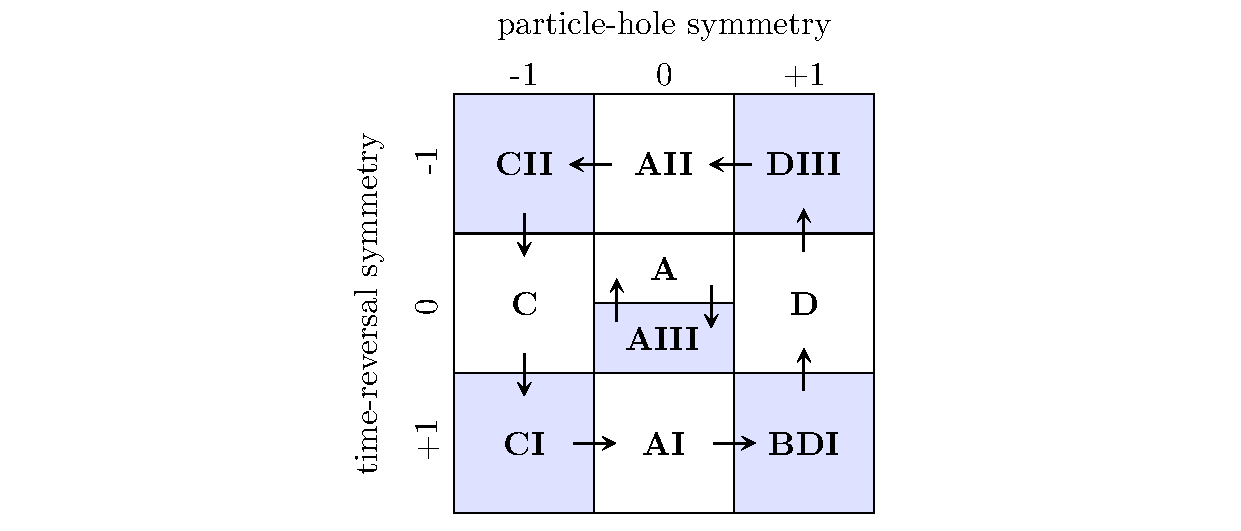
\includegraphics[width = 0.95\textwidth]{intro-bclock.pdf}
\caption[The Bott clock]{The Bott clock~\cite{10foldKitaev2009}. Light blue color labels the chiral classes and the arrows show the direction in which dimensional extension $d \rightarrow d+1$ conserves the topological classification. The complex classes are located in the center of the table and have a periodicity of two, while the real classes (with periodicity of eight) are represented around the clock.}
\label{fig:bottclock}
\end{figure}

It is important to note that while all these properties are formally derived relying on the clean, periodic Hamiltonians, the topological classification is robust against any small perturbations preserving the gap, including the effect of disorder.

\section{Bulk-boundary correspondence}
Up to now, we have observed that systems can be classified into distinct symmetry classes based on their bulk properties. In reality, boundary effects are inevitable due to finite sizes of samples. A striking feature of non-interacting fermionic systems\footnote{Indeed, this is a rather generic property of free fermions. The toric code, for instance, is a topologically ordered phase, but has no gapless excitations on the boundary.} is that the bulk topology is intimately connected to the edge physics. More precisely, opening the boundaries of an initially periodic system with assigned non-zero topological invariant results in the presence of robust boundary modes\footnote{Given that the symmetries required to protect a topological phase are still preserved on the boundary.}. These modes survive any small local perturbations of the Hamiltonian as long as the topological properties of the bulk are not affected. This observation is the essence of the \emph{bulk-boundary correspondence}.
 
The first instance of the correspondence between bulk and boundary appeared in the context of anomalies in quantum field theory, with the prominent example of the Adler–Bell–Jackiw anomaly for chiral fermions~\cite{NIELSEN1983389}. It was observed that the effective field theories for bulk and boundary degrees of freedom, when defined separately, lead to quantum anomalies. To overcome the issue, both bulk and boundary have to be treated simultaneously and therefore the anomalies cancel out. Despite a lack of general proof\footnote{Probably the most general proof was presented in Ref.~\cite{PhysRevLett.71.3697} for IQH systems.}, the bulk-boundary correspondence has been rigorously studied in several symmetry classes~\cite{doi:10.1142/S0129055X02001107, doi:10.1143/JPSJ.81.114602, LORING2015383, Graf2013}.

\begin{figure}[H]
\centering
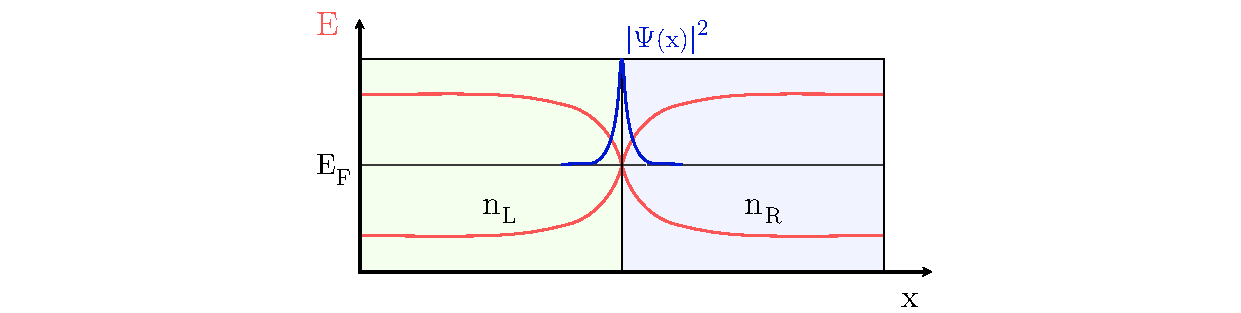
\includegraphics[width = \textwidth]{intro_bbc.pdf}
\caption[Schematic representation of the bulk-boundary correspondence]{Schematic representation of the bulk-boundary correspondence. If two systems $L$ and $R$, characterized by the invariants $n_L$ and $n_R$ ($n_L \neq n_R$), are joined at interface, there have to be gapless states localized at a domain wall associated with a band gap closing. The number of boundary states is determined by the difference $|n_L  - n_R|$.}
\label{fig:bbc}
\end{figure}

An heuristic explanation behind the correspondence is the following. Suppose we have two semi-infinite systems $L$ and $R$, illustrated in Fig.~\ref{fig:bbc}. The systems belong to the same symmetry class (thus are characterized by the index $n$), but the values of their invariants are different, $n_L \neq n_R$. As a topological invariant can only change if the bulk gap closes and no relevant symmetries are broken, a topological phase transition between two distinct gapped systems must be accompanied by the local gap closing. As a consequence, gapless states localize at the interface of the two materials and their number depends on the difference between indices $|n_L  - n_R|$. In particular, this relation holds for a single sample with a non-zero topological invariant, where the edge modes appear at the border with trivial (by definition) vacuum.

Most often, the bulk-boundary correspondence refers to the relation between $d$-dimensional bulk and boundary modes in $(d-1)$-dimensions~\cite{prodan2016bulk}. However, topological line and point defects can be also predicted from the periodic table~\cite{PhysRevB.82.115120}. A new type of the correspondence was established for the so-called higher-order topological insulators, in which the boundary states are manifested in codimensions $(d-D)$, with $ D>1$~\cite{HOTI12018}.

\section{Geometric phases}
\label{sec:geometric_phase}
For a long time, the importance of the phase factor associated with an adiabatic evolution of a quantum state was rather overlooked. However, if a cyclic evolution is considered, an accumulated phase can have a purely geometric character with potentially observable consequences. This phase factor is known as the Berry phase~\cite{berry84}. 
\subsection{Introduction to the Berry phase}
To explain the concept of the Berry phase, consider a system that has an implicit dependence on some external parameter $\mathbold{\xi}$. The parameter $\mathbold{\xi}$ may, in general, vary in time and the Hamiltonian is then $H(\mathbold{\xi} (t))$. According to the adiabatic theorem, a physical system initially in an eigenstate $\ket{\psi_n (0)} = \ket{ n ( \mathbold{\xi} (0))}$ will remain in its instantaneous eigenstate if a given perturbation is acting on it slowly enough
\begin{equation}
H(\mathbold{\xi} (t))  \ket{ n ( \mathbold{\xi} (t))} = E_n (\mathbold{\xi} (t))  \ket{ n ( \mathbold{\xi} (t))}.
\label{eq:adiabatic_ev}
\end{equation}
During the adiabatic evolution, the state does not only acquire a standard time-dependent phase, but also an extra phase factor $\gamma_n$
\begin{equation}
\ket{\psi_n (t)} = \exp \left( \mathrm{i} \gamma_n (t) \right) \exp \left( - \frac{\mathrm{i}}{\hbar} \int_0^t \epsilon_n (\mathbold{\xi} (t')) \, dt' \right)  \ket{ n ( \mathbold{\xi} (t))}.
\label{eq:phases_adiabatic}
\end{equation}
The phase factor $\gamma_n$ can be written as
\begin{equation}
\gamma_n = \int_C \bm{\mathcal{A}}_n (\mathbold{\xi}) \, d \mathbold{\xi}; \hspace{1cm}  \bm{\mathcal{A}}_n  ( \mathbold{\xi} ) = \mathrm{i} \braket{ n ( \mathbold{\xi} ) | \frac{\partial}{\partial \mathbold{\xi} } | n ( \mathbold{\xi} )}, 
\label{eq:berry_phase1}
\end{equation}
where $\bm{\mathcal{A}}_n$ is the gauge-dependent connection and $C$ denotes the contour along which the parameter $ \mathbold{\xi}$ evolved. After performing a $\mathrm{U}(1)$ gauge transformation, the connection and the state transform according to
\begin{equation}
\begin{aligned}
\ket{ n ( \mathbold{\xi} (t))}  \rightarrow & \ket{ n' ( \mathbold{\xi} (t))} = e^{\mathrm{i} \varphi ( \mathbold{\xi})}  \ket{ n ( \mathbold{\xi} (t))}, \\
 \bm{\mathcal{A}}_n  \rightarrow & \bm{\mathcal{A}}'_n = \bm{ \mathcal{A}}_n  - \frac{\partial}{\partial  \mathbold{\xi}} \varphi (  \mathbold{\xi} ).
\end{aligned}
\label{eq:berry_gaugetransform}
\end{equation}
These equations exactly correspond to the gauge freedom of the vector potential in an electromagnetic field. It should not come as a surprise as the Berry phase and its connection exactly matches the phase picked up by an electron moving in a magnetic field, the so-called Aharonov-Bohm effect. 

Let $ \mathbold{\xi} (0) $ and $  \mathbold{\xi} (t_F)$ be the endpoints of the contour $C$. If $ \mathbold{\xi} (0) \neq \mathbold{\xi} (t_F)$, that is the evolution does not follow a closed contour, $\varphi$ can be chosen in a way that $\gamma_n$ vanishes. On the other hand, if a cyclic evolution is considered (so $ \mathbold{\xi} (0) = \mathbold{\xi} (t_F)$), there is a constraint for the values of $\varphi$ arising from the gauge transformation of the wave function in Eq.~\eqref{eq:berry_gaugetransform}
\begin{equation}
\varphi ( \mathbold{\xi} (0)) - \varphi ( \mathbold{\xi}  (t_F) ) = 2 \pi m, \hspace{1cm} m \in \mathbb{Z}.
\end{equation}
Therefore, the phase $\gamma_n$ called \emph{the Berry phase} 
\begin{equation}
\gamma_n = \oint_C \bm{\mathcal{A}}_n (\mathbold{\xi}) \, d \mathbold{\xi}
\label{eq:berry_phase_final}
\end{equation}
becomes finite and well-defined. 

\subsection{Berry phases in band theory}
The Berry phase effects can be naturally studied in the context of band theory as they are directly connected to the electronic properties of a system~\cite{RevModPhys.82.1959}. The parameter space is therefore the reciprocal space, with a set of Bloch states $\ket{\psi_{n \mathbf{k}}}$ at each $\mathbf{k}$ momentum. For a single, isolated band $n$, we can rewrite a connection $\bm{\mathcal{A}_n}$ in Eq.~\eqref{eq:berry_phase1} in $\mathbf{k}$-space
\begin{equation}
\bm{\mathcal{A}_n} ( \mathbf{k}) = \mathrm{i} \braket{u_{n \mathbf{k}} | \nabla_{\mathbf{k}} | u_{n \mathbf{k}}}, 
\label{eq:berry-conn}
\end{equation}
which is known as the Berry connection. Note that we use the lattice-periodic part of a Bloch eigenstate, $\ket{u_{n \mathbf{k}}}  = e^{- \mathrm{i} \mathbf{k} \cdot \mathbf{r}} \ket{\psi_{n \mathbf{k}}}$, as its derivative $\partial_{k} \ket{u_{n \mathbf{k}}}$ behaves well and spans the same Hilbert space as $\ket{u_{n \mathbf{k}}}$. The form of $\bm{\mathcal{A}}$ resembles the electromagnetic vector potential and it is also gauge-dependent. In analogy to the magnetic field, we can define the Berry curvature
\begin{equation}
\bm{\mathcal{F}} ( \mathbf{k}) =  \nabla_{\mathbf{k}} \times \bm{\mathcal{A}} ( \mathbf{k}),
\label{eq:berry-curv}
\end{equation}
which is gauge invariant. Extending the considerations to the case of $N$ bands separated from the rest of the spectrum results in the non-Abelian generalization of Eqs.~\eqref{eq:berry-conn} and~\eqref{eq:berry-curv}
\begin{equation}
\begin{aligned}
&\hspace*{1cm}\bm{\mathcal{A}} ( \mathbf{k})_{mn, \mu}  =  \mathrm{i} \braket{ u_{m \mathbf{k}} | \partial_{k_{\mu}} |  u_{n \mathbf{k}}}, \\
\bm{\mathcal{F}}_{m n, \mu \nu} ( \mathbf{k}) = \mathrm{i} & \left( \braket{ \partial_{k_{\mu}} u_{n \mathbf{k}} | \partial_{k_{\nu}}   u_{m \mathbf{k}}}  - \braket{ \partial_{k_{\nu}} u_{n \mathbf{k}} | \partial_{k_{\mu}} u_{m \mathbf{k}}} - [ \bm{\mathcal{A}}_{\mu},  \bm{\mathcal{A}}_{\mu}]_{mn}} \right) .
\end{aligned}
\end{equation}
Remarkably, the Berry phase of the electronic wavefunctions and associated quantities -- curvatures and connections -- allow to compute the macroscopic polarization, which underlies the formulation of the modern theory of polarization~\cite{resta2007theory}. As in the case of the Gaussian curvature in the Eq.~\eqref{eq:gaussbonnet}, an integral of the Berry curvature $\bm{\mathcal{F}} ( \mathbf{k})$ over the BZ should give an integer. In two dimensions, the corresponding topological invariant is the (first) Chern number $C$
\begin{equation}
C = \frac{1}{2 \pi}  \int_{\mathrm{BZ}} d\mathbf{k} \, \bm{\mathcal{F}}  (\mathbf{k}).
\label{eq:chern_number}
\end{equation}
If $\bm{\mathcal{F}} (\mathbf{k})$ is a continuous function, then the Chern number vanishes. This indicates that the Chern number is associated with a non-trivial structure of the Berry curvature of a band. 

The eigenstates obtained from a numerical diagonalization of the Hamiltonian $\mathcal{H} (\mathbf{k})$ yield random phases at different $\mathbf{k}$-points on the finite mesh. A particularly useful, gauge-invariant expression for the Chern number of the $n$th band is based on the Kubo formula
\begin{equation}
C_n = \frac{\mathrm{i}}{2 \pi} \int_{\mathrm{BZ}} d \mathbf{k} \sum_{n \neq m}  \frac{ \braket{ u_{n \mathbf{k}} | \partial_{k_x} \mathcal{H} (\mathbf{k}) | u_{m \mathbf{k}}} \braket{ u_{m \mathbf{k}} | \partial_{k_y} \mathcal{H} (\mathbf{k}) | u_{n \mathbf{k}} } - (n \leftrightarrow m)  }{ \left( E_{n \mathbf{k}} - E_{m \mathbf{k}} \right)^2},
\label{eq:chern-kubo}
\end{equation}
where $E_{n \mathbf{k}}$ and $\ket{u_{n \mathbf{k}}}$ are, respectively, the energies and eigenstates of $\mathcal{H} (\mathbf{k})$. The total Chern number of a multiband system is a sum over all occupied states $n$
\begin{equation}
C = \sum_{n \in \mathrm{occ}} C_n.
\end{equation}

As we will see in Section~\ref{sec:iqhe}, the Chern number is directly connected to the experimentally observed quantization of the Hall conductivity.

\section{Topical examples}
\label{sec:examples}
In order to give a more concrete footing to the notions introduced in this Chapter, we present a short overview of several models belonging to different symmetry classes. The goal is to explain how topology is connected to physically demonstrated phenomena. We start with the integer quantum Hall effect and Chern insulators (especially the Haldane model) as representatives of the symmetry class A. We then discuss topological insulators with time-reversal symmetry characterized by $\mathbb{Z}_2$ invariants, in particular the Kane-Mele model as a prototypical example. In the end, we discuss the role of the chiral symmetry in the one-dimensional Su-Schrieffer-Heeger model in the BDI class.

\subsection{Integer quantum Hall effect}
\label{sec:iqhe}
To begin with, consider a two-dimensional system in the $xy$-plane, exposed to a fixed magnetic field in the $z$-direction, $\mathbf{B}  = B_z \mathbf{e}_z$. We can then study the 2D current densities $\mathbf{j}$ and electric fields $\mathbf{E}$, which are related by Ohm's law
\begin{equation}
\mathbf{j} = \begin{pmatrix}
\sigma_{xx} &  \sigma_{xy} \\
\sigma_{yx} & \sigma_{yy}
\end{pmatrix}
\begin{pmatrix}
E_x \\ E_y
\end{pmatrix} = \sigma \mathbf{E}, \hspace*{1cm} \mathbf{E} = \begin{pmatrix}
\rho_{xx} &  \rho_{xy} \\
\rho_{yx} & \rho_{yy}
\end{pmatrix}
\begin{pmatrix}
J_x \\ J_y
\end{pmatrix} = \rho \mathbf{j}.
\end{equation}
The resistivity\footnote{Resistivity is defined as the ratio of the product of the resistance and area to the length of the conductor. In two dimensions, both resistivity and resistance have the same dimension. This also applies to the conductivity/conductance.} matrix $\rho$ is the inverse of the conductivity $\sigma$, $\rho \cdot \sigma = 1$. For an isotropic sample, we can assume that $\sigma_{xx} = \sigma_{yy}$ and $\sigma_{yx} = - \sigma_{xy}$ (and similarly for the conductance). In the classical Hall effect setup, the charge carriers (holes or electrons) with current density $\mathbf{j} = j_x \mathbf{e}_x$ are affected by the Lorentz force $\mathbf{F}_l = q ( \mathbf{v} \times \mathbf{B} )$, leading to an electric field $\mathbf{E} = E_y \mathbf{e}_y $ in the transverse direction to the current. Using the Drude model~\cite{kittel1968introduction}, one can show that the Hall resistivity is related linearly to the applied magnetic field
\begin{equation}
\rho_{xy} =  B_z  \mathcal{R}_H = - \frac{B_z}{ne},
\end{equation}
where we assumed the carriers to be electrons. The Hall coefficient $ \mathcal{R}_H  = -1/ne$ is a material dependent parameter, where $n$ is the electron density and $e$ is the elementary charge. The classically derived formula breaks down in the low-temperature, high-magnetic field regime, where quantum effects play a substantial role. The discovery of the quantum Hall effect by von Klitzing and co-workers~\cite{IQHE1980} paving the way to the studies of topological phenomena was that $\rho_{xy}$ is not proportional to $B_z$ anymore, but has plateaus at quantized values
\begin{equation}
\rho_{xy} = \frac{1}{\nu} \frac{h}{e^2},
\label{eq:hallres}
\end{equation}
while both the longitudinal resistance $\sigma_{xx}$ and conductivity $\rho_{xx}$ vanish. This is possible because of the matrix formulation of $\sigma$ and $\rho$. Therefore, the Hall conductivity and resistivity are related by $\sigma_{xy} \cdot \rho_{xy} = -1$, leading to $\sigma_{xy} = \nu e^2 /h$. The vanishing conductivity $\sigma_{xx}= 0$ means that a quantum Hall system is an insulator parallel to the electric field, while the vanishing resistivity $\rho_{xx} = 0$ means that there is no voltage drop parallel to the current. For the integer quantum Hall effect, $\nu$ is an integer. 

\subsubsection{Quantum picture}
The quantum treatment of the IQHE starts with a simple Hamiltonian for a two-dimensional electron gas (2DEG) in a magnetic field $\mathbf{B} = B \mathbf{e}_z$. We neglect the interactions between electrons and focus on the single-particle description. In the Landau gauge, the electromagnetic vector potential is $\mathbf{A} = Bx \mathbf{e}_y$ satisfying $\nabla \times \mathbf{A} = \mathbf{B}$. A minimal coupling to the electromagnetic field is taken into account by the substitution of the momentum operator $ \mathbf{p} \rightarrow  \mathbf{p}  + e \mathbf{A} $. Hence, the Hamiltonian for a non-interacting, non-relativistic 2DEG becomes
\begin{equation}
H = \frac{\hbar}{2 m^*} ( \mathbf{p}  + e \mathbf{A} )^2 = \frac{\hbar}{2m^*} p_x^2 + \frac{\hbar}{2m^*} (p_y +  eBx)^2.
\label{eq:H-iqhe}
\end{equation}
Here, $m^*$ denotes the renormalized effective mass. The Hamiltonian in Eq.~\eqref{eq:H-iqhe} is translationally invariant in the $y$-direction and therefore commutes with the momentum operator $p_y$. As a consequence, the eigenstates of $H$ can be chosen to be the eigenstates of $p_y$ and $p_y$ can be replaced by its eigenvalues $\hbar k_y$ and $H$ can be rewritten as
\begin{equation}
H = \frac{1}{2m^*} p_x^2 + \frac{1}{2} m^* \omega_c^2 ( x + k_y l_B^2)^2,
\end{equation}
where $\omega_c = eB/m$ is the cyclotron frequency and $l_B = \sqrt{ \hbar / eB}$ is the magnetic length. $\sqrt{2} l_B$ can be seen as the radius of the electron orbits in the semiclassical picture. The Hamiltonian resembles a quantum harmonic oscillator with a potential shifted by $-k_y l_B^2$, which has its energy eigenvalues of the form 
\begin{equation}
E_n = \hbar \omega_c \left( n + \frac{1}{2} \right), \hspace*{0.5cm } n \in \mathbb{N}
\end{equation}
called the Landau levels. These energy levels are highly degenerate and the number of states per level $N_L$ can be approximated as
\begin{equation}
N_L \approx \frac{A}{2 \pi l_B^2 } = \frac{\Phi}{\Phi_0}
\end{equation}
with $\Phi_0 = h /e$ the quantum of flux and $\Phi = A B$ the total flux through the sample of area $A$. The Landau levels are similar to the energy bands in a band insulators. They are separated by a finite gap and the chemical potential can be tuned to lie in the gap. In the presence of a confining potential, the bulk of these Landau levels stay unchanged (corresponding in the classical picture to electrons orbiting in the bulk of the system), while at the edges, they are strongly deformed, with an energy following the form of the confining potential (consult Fig.~\ref{fig:LL}). By fixing the chemical potential $\mu$ to be in between two of the flat bulk Landau levels, it will now also cross exactly once (at each edge) each of the occupied Landau levels. Each crossed Landau level acts as a band in a typical metal or band insulator, and will therefore contribute exactly one unit $e^2/h$ of conductance. The total $\sigma_{xy}$ therefore measures the number of occupied bands. This correspond to the observed plateau of the Hall resistance as the conductance is left unchanged as long as the chemical potential does not cross another Landau level. 

\begin{figure}
\centering
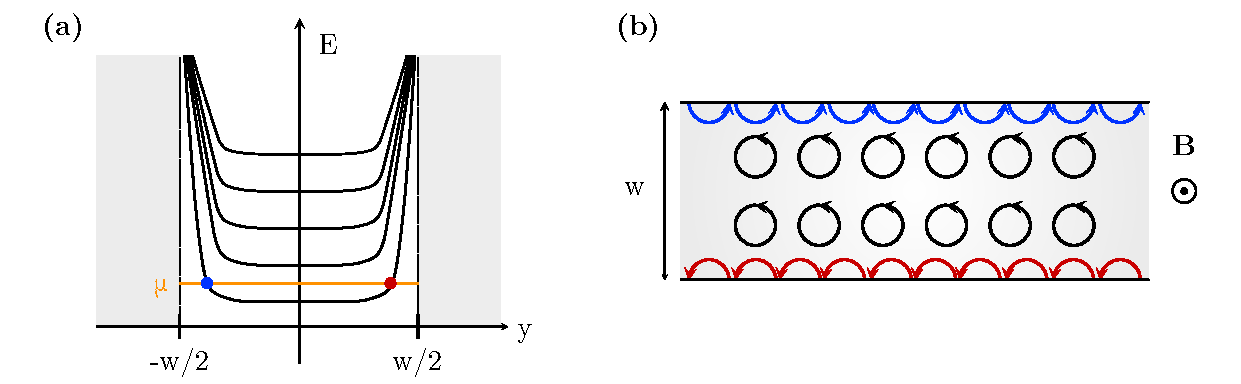
\includegraphics[width=0.9\textwidth]{intro-landau.pdf}
\caption[The Landau levels in the confining potential and the semiclassical orbits]{\textbf{(a)} The Landau levels in a confining potential and \textbf{(b)} the semiclassical cyclotron orbits. If the chemical potential $\mu$ is fixed between two Landau levels, the system remains insulating in the bulk, which corresponds to the closed cyclotron orbits. At the boundaries, however, gapless edge states appear due to the Landau levels bending. The edge states can be schematically represented as cyclotron orbits bouncing on the interfaces, each carrying the current in a single direction.}
\label{fig:LL}
\end{figure}

\subsubsection{Quantized Hall conductance and the Chern number}
We see that the Landau levels picture provides an intuitive explanation of the experimentally observed plateaus. However, it does not tell why the exact quantization is robust and occurs in the QH systems regardless of the microscopic details such as disorder or the geometry of a sample. The link to a topological origin of the quantization was first made by Laughlin based on a gauge argument~\cite{PhysRevB.23.5632}. Subsequently, Thouless, Kohmoto, Nightingale, and den Nijs (TKNN)~\cite{PhysRevLett.49.405}, in parallel to Avron, Seiler, and Simon~\cite{PhysRevLett.51.51}, related the Hall conductivity to the sum of the Chern numbers of all occupied bands times the quantum of conductance $e^2 /h$. Starting from the Kubo formula of conductivity based on linear response theory (compare to Eq.~\eqref{eq:chern-kubo}), TKNN showed that the Hall conductivity can be expressed as
\begin{equation}
\sigma_{xy} = \frac{e^2}{h} \sum_{n \in \mathrm{occ}} C_n
\end{equation}
with $C$ defined as in Eq.~\eqref{eq:chern_number}. This formulation does not depend in any way on the energies of a system, but only on the Bloch wavefunctions.

The boundary modes arising from the confining potential or the boundary of the systems are actually topologically protected and related to a non-zero Chern number. This comes as another instance of the bulk-boundary correspondence. We pictorially present the band structure and a chiral edge state in a system with $C =1 $ in Figs.~\ref{fig:qheqshe}~(a) and~(c). In a quantum Hall system, the left and right propagating modes are protected against the backscattering as they are macroscopically spatially separated on opposite edges of the sample. 


%\begin{tabular}{|c|c|}
%\hline 
%Electromagnetism & Bloch function \\ 
%\hline 
%Vector potential $\mathbf{A}$ & Berry connection $\bm{\mathcal{A}} = \braket{u_{\mathbf{k}} | \mathrm{i} \nabla_{\mathbf{k}} | u_{\mathbf{k}}}  $ \\ 
%\hline 
%Aharonov-Bohm phase $\phi = e / \hbar \oint \mathbf{A} \cdot d \mathbf{r}$ & Berry phase $ \gamma = \oint \mathbf{A} \cdot d \mathbf{k}$ \\ 
%\hline 
%Magnetic field $\mathbf{B} = \nabla \times \mathbf{A}$ & Berry curvature $bm{\mathcal{F}} = \nabla_{\mathbf{k}}  \times \bm{\mathcal{A}} $ \\
%\hline
%Quantized magnetic flux $\Phi = n \frac{h}{e}$ & Quantized Hall conductivity $\sigma_{xy} = \nu \frac{e^2}{h}$ \\ 
%\hline 
%Magnetic monopole charge & Chern number \\ 
%\hline 
%\end{tabular} 



\subsection{Chern insulators}
\label{sec:ci}
Even with zero net magnetic field, the system can realize a non-zero Chern number. This gives rise to the notion of the Chern insulators (CIs), also known as the quantum anomalous Hall effect. Experimentally, the CIs have been realized in a magnetic topological insulator~\cite{Chang167}, but also in fermionic ultracold atoms~\cite{Jotzu2014} or classical wave systems~\cite{CIacustic2019}. The simplest Chern insulator is modeled by a two band Hamiltonian $\mathcal{H}( \mathbf{k} )$, whose general form is given by\footnote{In fact, any two-state Hermitian Bloch Hamiltonian admit such a representation.}
\begin{equation}
\mathcal{H}( \mathbf{k} ) =  d_0 (\mathbf{k}) \sigma_0 + \mathbf{d}( \mathbf{k} )  \boldsymbol{\sigma},
\label{eq:twoband}
\end{equation}
where $ \boldsymbol{\sigma} = (\sigma_x, \sigma_y, \sigma_z)$ are the Pauli matrices and $  \sigma_0 = \mathbb{1}_{2 \times 2}$. The three-dimensional $\mathbf{d}( \mathbf{k} )$ describes the internal structure of Bloch states, while the energies are given by $d_0(\mathbf{k}) \pm |d(\mathbf{k})|$. If the system is insulating, we can define a unit vector $\mathbf{n} ( \mathbf{k})$, which maps a point on a torus to a two-dimensional sphere $S^2$ known as the Bloch sphere.
\begin{equation}
\mathbf{n} (\mathbf{k} ) = \frac{\mathbf{d}( \mathbf{k} ) }{|\mathbf{d} (\mathbf{k})|}, \hspace*{1cm} \mathbf{n} : T^2 \rightarrow S^2.
\end{equation} 
The Chern number can be written as
\begin{equation}
C = \frac{1}{4 \pi} \int_{T^2} \mathbf{n} \cdot \left( \frac{\partial \mathbf{n} }{\partial k_x} \times \frac{\partial \mathbf{n} }{ \partial k_y} \right) \, d \mathbf{k},
\end{equation}
which has a simple interpretation: it measures how many times the $\mathbf{n}$ vector wraps around the sphere as we integrate over the BZ.

\subsubsection{Haldane model}
In the seminal paper~\cite{Haldane1988}, Haldane proposed a model to describe spinless electrons in a single honeycomb lattice with a staggered magnetic flux pattern that leads to zero net magnetic flux. In addition to NN hopping terms appearing in the tight-binding description of graphene, there are also NNN hoppings with complex phases (illustrated in Fig.~\ref{fig:haldane}~(a)). These Aharonov-Bohm phases arise due to the time-reversal breaking staggered flux pattern, which are incorporated in the Hamiltonian through a Peierls substition, $t_1 \rightarrow t_1, \, t_2 \rightarrow t_2 e^{\mathrm{i} \phi}$. The model can be written as
\begin{equation}
H_{\mathrm{Haldane}} = t_1 \sum_{\langle ij \rangle} c^{\dagger}_i c_j + t_2 \sum_{\langle \langle i j \rangle \rangle} e^{\pm \mathrm{i} \phi} c^{\dagger}_i c_j  + M \sum_i  \xi_i c^{\dagger}_i c_j +  \mathrm{h. c.}.
\label{eq:haldane}
\end{equation}
The last term with $\xi = \pm 1$ assigns the on-site energies $+M$ for sites of sublattice $A$ and $-M$ for sublattice $B$. Hence, a non-zero $M$ breaks inversion symmetry.

To represent the Hamiltonian in Eq.~\eqref{eq:haldane} in momentum space, we use the property defined in Eq.~\eqref{eq:twoband} with the following components of the $\mathbf{d} ( \mathbf{k})$ vector
\begin{equation}
\begin{aligned}
d_0 (\mathbf{k} ) & = 2 t_2 \cos \phi \left[\sum_i \cos (\mathbf{k} \cdot \mathbf{a}_i) \right], \\ 
d_x (\mathbf{k} ) &= t_1 \left[ 1 + \cos ( \mathbf{k} \cdot  \mathbf{a}_1 ) + \cos ( \mathbf{k} \cdot  \mathbf{a}_2 ) \right], \\
d_y (\mathbf{k} ) & = t_1 \left[ \sin (\mathbf{k}  \cdot \mathbf{a}_1 ) -  \sin (\mathbf{k}  \cdot \mathbf{a}_2 ) \right], \\
d_z (\mathbf{k} ) & = M - 2t_2 \sin \phi \left[ \sum_i \sin (\mathbf{k}  \cdot \mathbf{a}_i) \right].
\end{aligned}
\end{equation}
$\mathbf{a}_i$ are the lattice vectors connecting the next-nearest neighbors (see Fig.~\ref{fig:haldane}~(a)), which we choose to be 
\begin{equation}
\mathbf{a}_1  = a \, (1, 0), \hspace*{0.5cm} \mathbf{a}_2  = a \, \left( \frac{1}{2}, \frac{\sqrt{3}}{2} \right),  \hspace*{0.35cm} \mathrm{and} \hspace*{0.35cm} \mathbf{a}_3  = \mathbf{a}_1 - \mathbf{a}_2 = a \, \left( \frac{1}{2}, - \frac{\sqrt{3}}{2} \right).
\end{equation}
As far as the topology is concern, we can ignore the energy shift $d_0 (\mathbf{k} )$. Firstly, we point out that the terms $d_x (\mathbf{k} )$ and $d_y (\mathbf{k} )$ are time-reversal symmetric for any value of $\phi$. $d_z (\mathbf{k} )$, on the other hand, satisfies $d_z (\mathbf{k} ) = d_z (-\mathbf{k} )$ only for $ \phi = 0, \, \pi$. The gap closes if and only if $d_x = d_y = d_z = 0$. For $M=0$ and $\phi=0, \, \pi$, $d_z$ vanishes and the Hamiltonian is nothing but the celebrated low-energy graphene model. The gap then closes at the Dirac points $K$ and $K'$ (see Fig.~\ref{fig:haldane}~(b)) with a linear dispersion, forming two Dirac cones of opposite chirality. 

\begin{figure}[H]
\centering
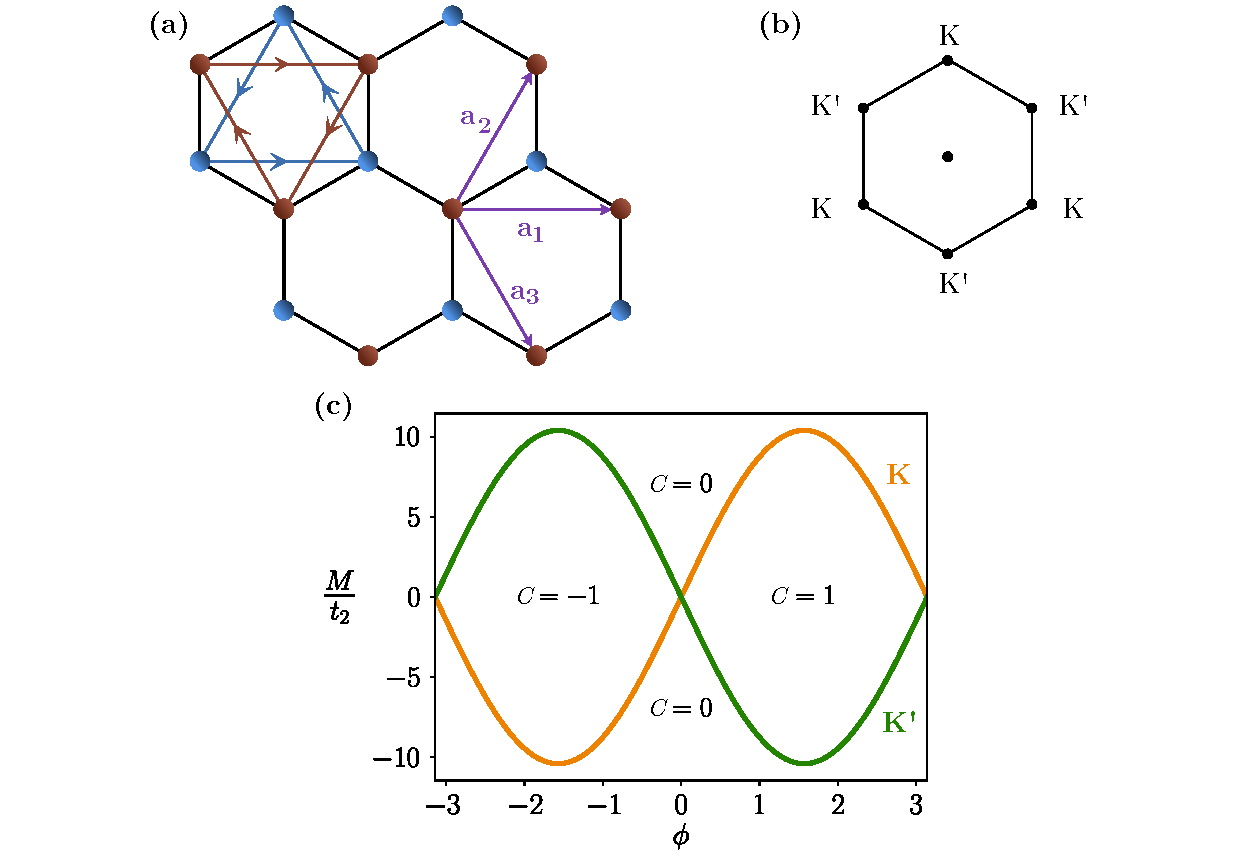
\includegraphics[width = 0.9\textwidth]{intro-haldane.pdf}
\caption[The Haldane model]{\textbf{(a)} Schematic representation of the Haldane model on the honeycomb lattice. The two sublattices, $A$ and $B$, are denoted by the blue and red colors, respectively. Next-nearest neighbor hoppings carry a phase $\phi$ with a sign $+$ ($-$) along blue (brown) links, resulting in the total zero flux. \textbf{(b)} The band gap closing occurs at the Dirac points $K = \left( \frac{2 \pi}{3 a}, \frac{2 \pi}{3 a \sqrt{3}} \right)$ and $K' = \left( \frac{2 \pi}{3 a}, -\frac{2 \pi}{3 a \sqrt{3}} \right)$ in the Brillouin zone. \textbf{(c)} The phase diagram on the plane $(\phi, M /t_2)$ with the Chern number of the lowest band. The gap closes at the critical lines $|M| = 3 \sqrt{3} t_2 \sin \phi$. Orange line corresponds to the band gap closing at the $K$ point, while green line to a band gap closing at the $K'$ point.}
\label{fig:haldane}
\end{figure}

For non-zero $M$ and $\phi$, the gap can still only close at the $K$ and $K'$ points. Therefore, it is convenient to work with a low-energy effective model. We can write the low energy expansion of the full Hamiltonian around the $K$ point as
\begin{equation}
\mathcal{H}_L (\mathbf{q}) = \hbar v_F \mathbf{q} \cdot \boldsymbol{\sigma}_{2D} + m \sigma_z
\label{eq:linear-H}
\end{equation}
where $\mathbf{q} = \mathbf{k} - K = (q_x, q_y)$, $\boldsymbol{\sigma}_{2D}  = (\sigma_x, \sigma_y)$, and $ m = d_z( K)$. The linearization leads to a massive Dirac Hamiltonian with mass $m$. A similar form emerges at the $K'$ point with a mass $m'$. For the Haldane model, the masses $m$ and $m'$ at $K$ and $K'$ points, respectively, are (with $ \hbar v_F = 1$)
\begin{equation}
m = d_z ( K) = M - 3 \sqrt{3} t_2  \sin \phi \hspace*{0.5cm} \mathrm{and} \hspace*{0.5cm}  m' = d_z ( K') = M + 3 \sqrt{3} t_2  \sin \phi.
\end{equation}

We can now construct the phase diagram with respect to the model parameters $(M, \phi)$. In a generic case, the system is an insulator, except when $|M| = 3 \sqrt{3} t_2  |\sin \phi| $. For $|M| > 3 \sqrt{3} t_2 | \sin \phi|$ both $K$ and $K'$ points have a mass of the same sign, hence the Hall conductivity vanishes and the system is in a trivial phase. Conversely, if $|M| < 3 \sqrt{3} t_2  | \sin \phi| $, then the Chern number is $\pm 1$, depending on the signs of $M$ and $\phi$. In the trivial phase, $m$ and $m'$ have the same sign, whereas in topological case $m = -m'$. Two insulating phases with different Chern numbers are separated by a semimetalic transition point with low-energy Dirac cones. Between a phase with a Chern number $\pm 1$ and the trivial phase with $C = 0$, the gap closes at a single $K$ point, and the system admits only a single Dirac cone. The two topological phases are separated by a graphene-like critical point with two Dirac cones. We illustrate the full phase diagram in Fig.~\ref{fig:haldane}~(c).

Here, a simple formula for the Chern number is
\begin{equation}
C = \frac{\mathrm{sgn} (m) - \mathrm{sgn} (m') }{2},
\end{equation}
which can be applied to any two bands model described by $\mathbf{d} ( \mathbf{k})$ vector, where the low-energy Hamiltonian is given by Eq.~\eqref{eq:linear-H} close to the gap closing momenta. Similar to the QHE, the edge states in the Haldane model are chiral, as depicted in Fig.~\ref{fig:qheqshe}~(c).

\subsection{Quantum spin Hall effect}
\label{sec:qshe}
Time-reversal symmetry breaking is an essential ingredient for the non-vanishing Hall conductivity $\sigma_{xy}$; the current $\mathbf{j}$ is odd under time-reversal, but the electric field $\mathbf{E}$ is even. However, the family of quantum Hall states can be extended by a new class of insulating states whose metallic edge modes are protected by the time-reversal symmetry, which was firstly theoretically proposed in graphene~\cite{KaneMeleGraphene,PhysRevLett.95.146802}\footnote{However, due to the negligible spin-orbit coupling and therefore small SOC-induced band gap $\sim 10^{-3}$ meV, it is not realizable experimentally under realistic conditions~\cite{PhysRevB.74.165310, PhysRevB.75.041401}.} and in strained zinc-blende semiconductors~\cite{BernevigQSHE2006}. The quantum spin Hall (QSH) effect was subsequently predicted in HgTe/CdTe quantum wells~\cite{Bernevig1757} and confirmed experimentally one year later~\cite{MolenkampQSHE2007}. 

\begin{figure}[H]
\centering
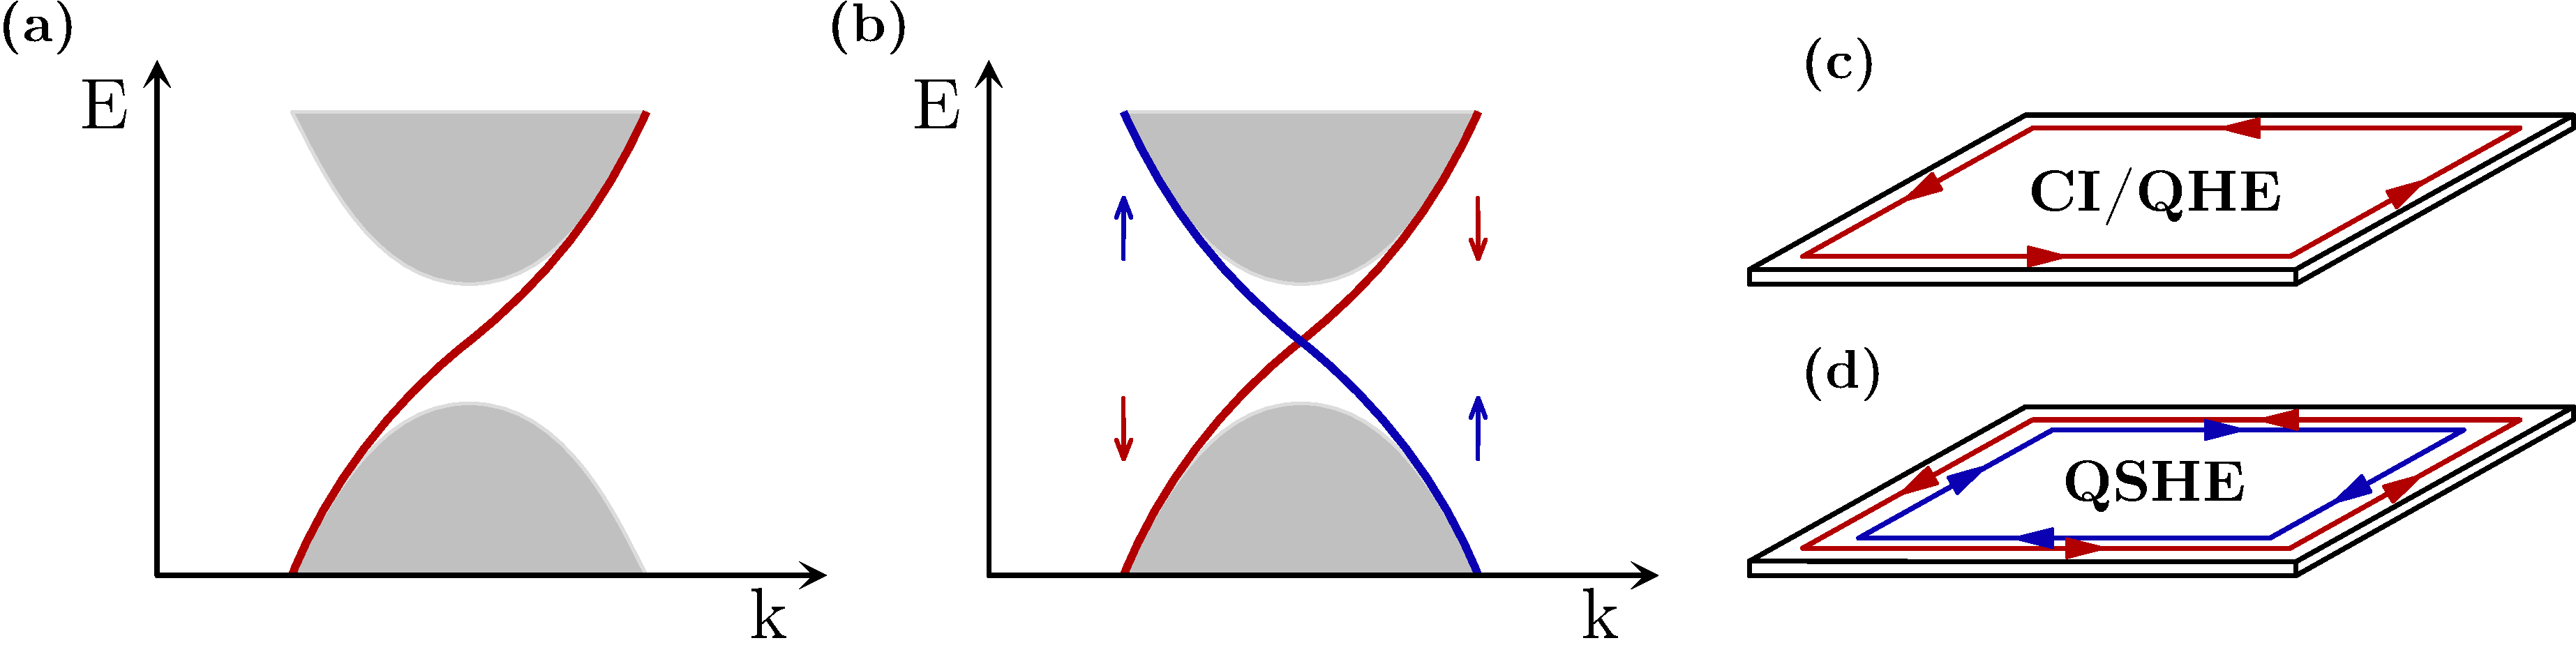
\includegraphics[width=\columnwidth]{intro_bs.pdf}
\caption[Comparison between a Chern insulator and a QSH system]{Schematic representation of the band structures of \textbf{(a)} a Chern insulator with $C = +1$ and \textbf{(b)} a quantum spin Hall system constructed as two copies of Chern insulators with opposite Chern numbers, together with conserved $z$-spin component. Edge states have \textbf{(c)} chiral character for a phase with broken time-reversal symmetry, while \textbf{(d)} TRS systems exhibit helical edge modes.}
\label{fig:qheqshe}
\end{figure}

In QSH systems, a pair of spin-polarized edge states counter-propagate along the boundary is usually referred to as \emph{helical} edge states (schematically depicted in Fig.~\ref{fig:qheqshe}~(d)). The helical boundary modes lead to a spin accumulation at the two edges transverse to the current direction rather than to a charge accumulation. The spin current $\mathbf{j}^S$ is even under TRS, which allows for the non-zero spin Hall conductivity $\sigma_{xy}^S$. In contrast to the charge current in QH systems, the spin current is not necessarily quantized~\cite{qsh-review, PhysRevB.100.245430}. Two edge modes within a helical pair are time-reversal conjugates of one another, forming a Kramers pair. The TRS symmetry $\mathcal{T}^2 = -1$ forbids the backscattering between states in a Kramers pair, which explains the robust nature of the edge states. As long as there are an odd number of Kramers pairs~\cite{PhysRevB.73.045322} and no magnetic impurities (breaking time-reversal symmetry), the edge spectrum is stable against disorder. The fact that TRS does not preclude an even number of Kramers pairs to couple and gap out explains why the topological invariant is taken modulo 2 and results in the $\mathbb{Z}_2$ classification.

\subsubsection{Kane-Mele model}
A canonical example of the QSH system is the Kane-Mele model~\cite{KaneMeleGraphene}, describing spinful electrons in a honeycomb lattice. The Hamiltonian $H_{\mathrm{KM}}$ in real space is given by
\begin{equation}
\begin{aligned}
H_{\mathrm{KM}} &= -t_1 \sum_{\langle i  j \rangle \alpha}  c_{i\alpha}^{\dagger} c_{j \alpha}  + \mathrm{i} \lambda_{\mathrm{SO}} \sum_{\langle \langle i j \rangle \rangle \alpha \beta} \nu_{ij} c_{i \alpha} ^{\dagger} \sigma_{\alpha \beta}^z c_{j \beta} \\
&+ \mathrm{i} \lambda_{\mathrm{R}} \sum_{\langle i j \rangle \alpha \beta} c_{i \alpha}^{\dagger} \left( \boldsymbol{\sigma}_{\alpha \beta} \times \mathbf{\hat{d}}_{ij} \right)_z c_{j \beta} + \lambda_{\mathrm{v}} \sum_{i \alpha} \xi_i c_{i \alpha}^{\dagger} c_{i, \alpha}.
\label{eq:km}
\end{aligned}
\end{equation}
The first term corresponds to the hopping between nearest-neighbors with strength $t_1$. The second term $\lambda_{\mathrm{SO}}$ is the mirror-symmetric spin-orbit coupling with spin-dependent NNN hopping. The coefficients $\nu_{ij} = (2 / \sqrt{3}) ( \mathbf{\hat{d}}_1 \times \mathbf{\hat{d}}_2 )$ are equal to $\pm 1$ with a sign that depends on whether a particle traverse from $i$ to $j$ clockwise ($\nu_{ij} = +1$) or counterclockwise ($\nu_{ij} = -1$), as in the Haldane model (consult Fig.~\ref{fig:haldane}~(a)). The third term $\lambda_{\mathrm{R}}$ describes the Rashba-type spin-orbit coupling. Here, $\boldsymbol{\sigma}$ stands for the vector of Pauli matrices $\bm{\sigma} = (\sigma_x, \sigma_y, \sigma_z)$, acting on the spin degrees of freedom denoted by the $\alpha$ and $\beta$ indices. Finally, the last term $ \lambda_{\mathrm{v}}$ is a staggered sublattice potential with $ \xi_i= 1$ for the $A$ sublattice and $-1$ for the $B$ sublattice. Non-zero $\lambda_{\mathrm{SO}}$ term breaks the $\mathrm{SU} (2)$ spin symmetry down to $\mathrm{U}(1)$ (conservation of the total spin polarization along the $z$ axis). The Rashba term breaks it further into a discrete $\mathbb{Z}_2$ symmetry (parity of the total spin polarization along the $z$ axis) and, in addition, breaks the mirror symmetry $z \rightarrow -z$. Introducing a finite $ \lambda_{\mathrm{v}}$ leads to the breaking of the inversion symmetry $\mathcal{I}$ and the opening a trivial gap.

The system can be understood from the simple limit $\lambda_{\mathrm{R}} = 0$. Then, the Kane-Mele model is basically two copies of the Haldane model with opposite chiralities and conserved spin component $S_z$ pointing out of the 2D plane (consult Fig.~\ref{fig:qheqshe}). Conveniently, the momentum-space Hamiltonian can be then written in a block-diagonal form
\begin{equation}
\mathcal{H}_{\mathrm{KM}} ( \mathbf{k}) = \begin{pmatrix}
\mathcal{H}_{\uparrow} ( \mathbf{k}) & 0 \\
0 & \mathcal{H}_{\downarrow} ( \mathbf{k})
\end{pmatrix}.
\label{eq:KM_Bloch_copies}
\end{equation}
In TRS systems, the total Chern number at half-filling always vanishes, however it is possible to assign a non-zero $C$ to the spin sectors separately. Each band is doubly degenerate, \ie spin-up and spin-down states have the same energy, which therefore leads to the constraint $C_{\uparrow} = - C_{\downarrow}$ as their sum must vanish. 

\hspace{-0.5cm}We can then define the spin Chern number~\cite{ShengCs2006}
\begin{equation}
C_s = \frac{C_{\uparrow} - C_{\downarrow}}{2}.
\label{eq:spinchern}
\end{equation}
In the presence of any spin-nonconserving processes, it is not possible to compute separately the Chern number of each spin flavour, thus the definition of $C_s$ in Eq.~\eqref{eq:spinchern} breaks down. However, time-reversal symmetry allows to define a more general $\mathbb{Z}_2$-valued invariant. 

\subsubsection{$\mathbb{Z}_2$ invariant}
There exist several expressions for the $\mathbb{Z}_2$ invariant. Historically, the first formulation was given by Kane and Mele~\cite{PhysRevLett.95.146802}, where they interpreted the non-zero $\mathbb{Z}_2$ index as an obstruction to define a smooth gauge over the whole BZ. The idea is to consider the Pfaffian Pf of the antisymmetric matrix $m$ connecting the Bloch states $\ket{u_j (\mathbf{k})}$ with their partners related by the time-reversal symmetry $\Theta$
\begin{equation}
m_{ij} ( \mathbf{k} ) = \braket{u_i ( \mathbf{k} ) | \Theta |  u_j (\mathbf{k}) },
\label{eq:z2_m-matrix}
\end{equation}
with $i, \, j$ labeling the occupied states. The matrix $m$ is not unitary, but antisymmetric $m^{\mathrm{T}} (\mathbf{k}) = - m (\mathbf{k})$. Moreover, the number of filled bands is always even due to time-reversal symmetry, hence the Pfaffian is well-defined. Recall that the Pffafian $\mathrm{Pf} (A)$ of a $2n \times 2n$ skew-symmetric matrix $A$ is defined as
\begin{equation}
 \mathrm{Pf} (A) = \frac{1}{2^n n!} \sum_{ \mathcal{P}} \mathrm{sgn} ( \mathcal{P} ) \prod_{i = 1}^n A_{\mathcal{P} ( 2i - 1) \mathcal{P} ( 2i)},
\end{equation}
where the summation is over all permutations $\mathcal{P}$ of its indices and the permutation group has $2n$ elements. The Pfaffian of $A$ verifies $( \mathrm{Pf} (A))^2 = \det A$. 

The zeros of Pf$(m)$ correspond to phase vortices that can only occur in isolated points in the BZ and always come in pairs as $|\mathrm{Pf} (m(\mathbf{k}))| = |\mathrm{Pf} (m(-\mathbf{k}))|$, except at the \emph{time-reversal invariant momenta} (TRIMs). These momenta are special points $\Gamma_i$ in the BZ satisfying $\Gamma_i + G = - \Gamma_i$ for a reciprocal lattice vector $G$, \ie the TRS maps them onto themselves. We represent TRIMs in two- and three-dimensional BZ in Fig.~\ref{fig:TRIMs}. 

\begin{figure}[H]
\centering
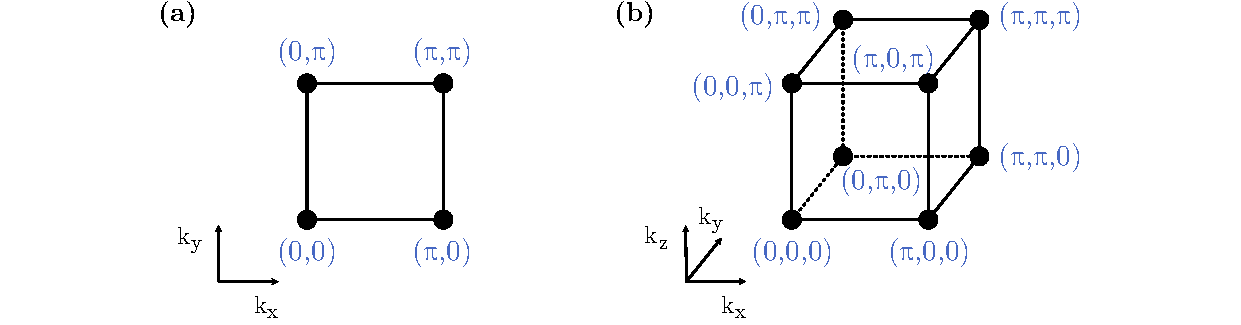
\includegraphics[width =\textwidth]{into_bz.pdf}
\caption[Time-reversal invariant momenta in two- and three-dimensional Brillouin zone]{Time-reversal invariant momenta in \textbf{(a)} two- and \textbf{(b)} three-dimensional Brillouin zone for a square or cubic lattice.}
\label{fig:TRIMs}
\end{figure}

At TRIMs, all bands exhibit Kramers' degeneracy. The subspace spanned by occupied Bloch states $\ket{u_i ( \mathbf{k} ) }$ is the same as for their $\Theta \ket{ u_i (\mathbf{k})}$ partners, hence the Pfaffian has unit modulus $|\mathrm{Pf} (m(\Gamma_i))| = 1$. Now, the zeros of the Pfaffian can only be gapped out if two vortices are brought together. A single pair of vortices can only meet at a TRIM. However, as the Pfaffian is always of unit modulus there, the vortices cannot be supported and therefore cannot annihilate. On the other hand, two (or any even number of) pairs of vortices can always meet away from the TRIMs, and therefore be smoothly removed by a continuous deformation of the Hamiltonian. Consequently, the parity of the number of pairs of vortices of the Pfaffian $\mathrm{Pf}(m(\mathbf{k}))$ can serve as a $\mathbb{Z}_2$-valued topological invariant $\nu$.

As the time-reversal symmetry maps $\mathbf{k}$ to $-\mathbf{k}$, there is a redundancy in a description based on the whole BZ. Instead, one may define an effective Brillouin zone (EBZ), which includes only one state out of each Kramers pair $(\mathbf{k}, -\mathbf{k})$, excluding the boundary. Hence, we can compute the invariant $\nu$ that corresponds to the parity of the number of vortices in the EBZ 
\begin{equation}
\nu = \frac{1}{2 \pi \mathrm{i} } \int_{\partial \mathrm{EBZ}} d \mathbf{k} \nabla_{\mathbf{k}} \log ( \mathrm{Pf}( m(\mathbf{k}))) .
\end{equation}

A more practical expression of the $\nu$ invariant based on the sewing matrix $w$ was proposed by Fu and Kane~\cite{PhysRevB.74.195312} 
\begin{equation}
w_{ij} ( \mathbf{k} ) = \braket{u_i (\mathbf{-k} ) | \Theta|  u_j (\mathbf{k}) }.
\label{eq:z2_w-matrix}
\end{equation}
The matrix $w$ is unitary and, a priori, antisymmetric only at TRIMs, where it coincides with the $m$ matrix defined in Eq.~\eqref{eq:z2_m-matrix}. There, we can express the $\nu$ invariant as
\begin{equation}
(-1)^{\nu} = \prod_{i}  \delta_i  \hspace*{0.5cm}  \mathrm{with}  \hspace*{0.5cm}  \delta_i  =  \frac{\mathrm{Pf} (w ( \Gamma_i)) }{\sqrt{\det w (\Gamma_i) }} = \pm 1.
\label{eq:pfaffian-z2}
\end{equation}
If inversion symmetry is present, the expression further simplifies. Each Kramers pair $n$ has a well-defined parity $\xi_{2n} (\Gamma_i) = \xi_{2n- 1} (\Gamma_i)  = \pm 1$, thus
\begin{equation}
 (-1)^{\nu} = \prod_i \delta_i   \hspace*{0.5cm} \mathrm{with} \hspace*{0.5cm}  \delta_i = \prod_{n = 1}^N  \xi_{2n} (\Gamma_i).
\label{eq:fukane}
\end{equation}

\subsubsection{Topological insulators in three dimensions}
Both QHE and QSHE are intrinsically two-dimensional phenomena. However, according to the ten-fold way, the concept of time-reversal symmetric band insulators can be extended to three dimensions~\cite{PhysRevB.75.121306, PhysRevLett.98.106803}. For a $3D$ Brillouin zone, it is possible to define four $\mathbb{Z}_2$ invariants $(\nu_0; \nu_1, \nu_2, \nu_3)$, where $\nu_1, \nu_2, \nu_3$ are obtained by applying the formula in Eq.~\eqref{eq:pfaffian-z2} in each of the three planes $k_x k_y$, $k_x k_z$ and $k_y k_z$, fixing the remaining momentum to $\pi$, giving 16 topologically distinct phases in total. If all four invariants are even, the system is topologically trivial. The phases with $\nu_0 =1$ are said to be strong topological insulators, which have no analogy with 2D systems. It is in contrast to weak topological insulators with $\nu_0 =0$, but $\nu_i \neq 0$ for at least one $i \in \lbrace 1, 2, 3 \rbrace$. These phase can be regarded as a stacking construction of 2D layers and therefore require additional protection by a translation symmetry in the stacking direction. 

Apart from topological phase transition, 2D systems always have an even number of Dirac cones according to the \emph{fermion doubling theorem}\footnote{Nielsen-Ninomiya theorem states that in two dimensions, the chiral Dirac cones can only appear in pairs.}. In strong TIs, the pairs appear at two spatially separated surfaces such that there are an odd number of surface Dirac cones around the time-reversal invariant points of each surface Brillouin zone. The spin of these surface Dirac cones is locked to their momentum, a phenomenon known as the spin-momentum locking~\cite{RevModPhys.82.3045}.

\subsection{Su-Schriffer-Heeger chain}
\label{sub:ssh}
The Su-Schriffer-Heeger (SSH) model, firstly introduced to characterize the properties of the polyacetylene~\cite{SSH1976}, is a representative example of a topological system protected by the chiral symmetry\footnote{The SSH chain belongs to the BDI class, hence TRS and PHS are also present. However, they are not responsible for topological protection.}. The model describes a one-dimensional chain of spinless fermions, shown in Fig.~\ref{fig:ssh}~(a). A unit cell consists of two atomic species $A$ and $B$, connected by alternating hoppings $v$ and $w$. In real space, the Hamiltonian $H_{\mathrm{SSH}}$ is
\begin{equation}
H_{\mathrm{SSH}} =v \,  \sum_i  ( c_{i, \, A}^{\dagger} c_{i, \, B}  + \mathrm{h. c.})  +  w \,  \sum_i  ( c_{i + 1, \, A}^{\dagger} c_{i, \, B}  + \mathrm{h. c.} ),
\label{eq:ssh_realspace}
\end{equation}
where $v, \, w > 0 $ is assumed. There are two gapped phases with energy gap $\Delta E = 2 \, |v -w|$, separated by a gapless line at $v = w$. By defining the spinor $\Psi_k  = \left( c_{k A}, c_{k B} \right) $ acting on the sublattice degrees on freedom, we can represent the Hamiltonian from Eq.~\eqref{eq:ssh_realspace} in reciprocal space 
\begin{equation}
\mathcal{H}_{\mathrm{SSH}} (k) =  \sum_k  \Psi_k^{\dagger}  \begin{pmatrix}
0 & v + w e^{ \mathrm{i} k} \\
v + w e^{-\mathrm{i} k} & 0
\end{pmatrix}
\Psi_k.
\label{eq:ssh_bloch}
\end{equation}
The bulk dispersion relation reads $E_{\pm} (k) = \pm \sqrt{v^2 + w^2 + 2 v w \cos k}$ and the bulk gap closing occurs at $k = \pi$ for $w = v$. The SSH chain is a Hermitian two-band model, hence it can be expressed in terms of Pauli matrices as in Eq.~\eqref{eq:twoband}. The $\mathbf{d} (k)$ vector for the $\mathcal{H}_{\mathrm{SSH}}$ is therefore
\begin{equation}
\mathbf{d} (k) = \left( v + w \cos k \right) \, \sigma_x + \left( v \sin k \right) \, \sigma_y = d_x(k) \, \sigma_x  + d_y (k) \, \sigma_y.
\label{eq:ssh_pauli}
\end{equation}
The chiral symmetry $\mathcal{C} = \sigma_z$ constrains the values of $\mathbf{d} (k)$ vector to the $xy$-plane, so that $\mathbf{d} (k) = (d_x, d_y, 0)$ and $d_0 (k) = 0$. In the $d_x - d_y$ space, the $\mathbf{d} (k)$ vector traces a trajectory as the momentum $k$ varies from $0$ to $2 \pi$. This trajectory is necessarily closed due to the periodicity of the Brillouin zone. For a gapped system with $v < w$, the $\mathbf{d} (k)$ vector encloses the origin (corresponding to a gap closing point), whereas for an insulating phase with $v > w$ it does not. In fact, one cannot smoothly deform $\mathbf{d}(k)$ to go from a trajectory enclosing the origin to the one which does not without the closing the gap. 

The number of times $\mathbf{d}(k)$ winds around the origin, that is to say the \emph{winding number} $W$, therefore naturally arises as a relevant topological invariant. In general, the winding number can take any integer value, but for the SSH model is either $W= 1$ (if $v < w$) or $W = 0$ ($v > w$) as illustrated in Figs.~\ref{fig:ssh}~(d) and~(e). In the eigenbasis of the chiral symmetry $\mathcal{C}$, the Bloch Hamiltonian has a block off-diagonal structure
\begin{equation}
\mathcal{H} (k) = \begin{pmatrix}
0 & h( k) \\
h^* (k) & 0
\end{pmatrix}, \hspace*{0.5cm} h(k) = d_x (k) - \mathrm{i} d_y (k), 
\label{eq:H-Cbasis}
\end{equation}
which reduces the computation of the winding number $\nu$ to
\begin{equation}
W = \frac{\mathrm{1}}{2 \pi \mathrm{i}} \int_{0}^{2 \pi}  d k \,   \frac{\partial}{\partial k} \log h(k).
\label{eq:winding}
\end{equation}
A non-trivial bulk winding has also consequences on the spectrum in an open geometry. The phase with $W=1$ is characterized by the presence of a pair of edge modes at exactly zero energy, in contrast to the fully gapped system with $W = 0$, where all eigenstates uniformly spread over all lattice sites (see Figs.~\ref{fig:ssh}~(b) and~(c)). These edge states are therefore predicted by the topological invariant $W$. They will be gapped out only when the bulk gap closes, or when the chiral symmetry is broken. The breaking of chiral symmetry can be achieved, for instance by introducing long-range hoppings connecting the sites belonging to the same sublattice. Conversely, introducing longer range hoppings between sites of different sublattices allows for potentially higher winding numbers, and therefore more edge states if the TRS is also preserved.

\begin{figure}[H]
\centering
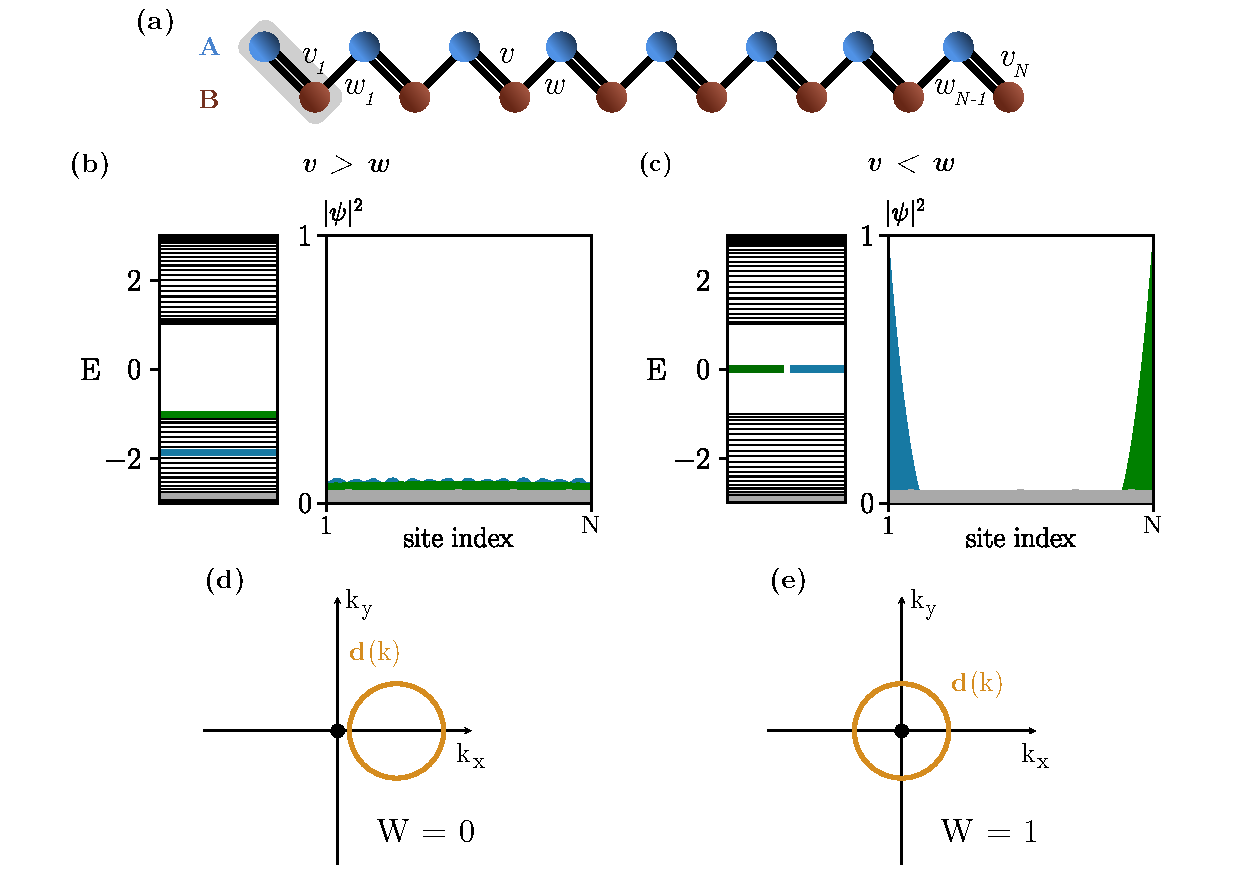
\includegraphics[width=\columnwidth]{intro_ssh.pdf}
\caption[The Su-Schriffer-Heeger model]{The Su-Schriffer-Heeger model. \textbf{(a)} schematic picture of a 1D chain. There are two inequivalent sublattices $A$ and $B$ (colored with blue and red, respectively) in a unit cell marked with a shaded area. Model has two type of hoppings: intracell with a strength $v$ and intercell denoted by $w$. \textbf{(b)} Energy spectra and \textbf{(c)} localization of representative eigenstates in two parameter regimes for the system with open boundary conditions. Depending on the values of $v$ and $w$, the model exhibits two topologically distinct phases: if $w < v$,  the system is in a trivial phase (with $w = 0$ as a fully dimerized case) and all states have bulk-like density profile shown in \textbf{(b)}. Conversely, if $w > v$, the system is in a topological phase with zero-energy gapless edge models (see \textbf{(c)}). Hybridization of the edge states is exponentially small in the system size. \textbf{(d)} and \textbf{(e)} are corresponding windings of the $\mathbf{d} (k)$-vector around the origin, which defines the bulk winding number $W$.}
\label{fig:ssh}
\end{figure}